\documentclass[a4paper,12pt]{report}
% es wurde leqno entfernt, da damit die Nummern von Gleichungen links standen
\usepackage{inputenc,fontenc}
\usepackage[a4paper,margin=3cm]{geometry}
\usepackage[english, german]{babel}
\usepackage[ngerman=ngerman]{hyphsubst}
% \usepackage{isodate}
\usepackage[hidelinks]{hyperref}
\usepackage{amsmath, amsfonts, amssymb, amsthm} %% mathematics tools
\usepackage{csquotes}
\usepackage[draft]{listofsymbols}
\usepackage[backend=biber, sorting=none, style=iso-numeric]{biblatex} %% Literature citing engine
\usepackage{subcaption}
\usepackage{graphicx}
\usepackage{algorithm}
\usepackage{algpseudocode}
\usepackage{dsfont} % für charakteristische 1
\usepackage{acro}

%%
%% Pflichtangaben -bitte hier einsetzen %%%%%%%%%%%%%%%%%%%%%%%%%%%%%%%%%%%%%%%%%%%%%%
%%
\newcommand{\name}{Göpel}
\newcommand{\vorname}{Noah}
\newcommand{\gebdatum}{01.02.2003}
\newcommand{\ort}{Riesa}
\newcommand{\betreuer}{Prof. Dr. Oliver Sander}
\newcommand{\institut}{Institut für Numerische Mathematik}
\newcommand{\thema}{Gewichtete Zählung von Eigenwerten auf einem Intervall}
\newcommand{\datum}{26.\ 09.\ 2024} %Format tt.\ mm.\ jjjj

%%%%%%%%%%%%%%%%%%%%%%%%%%%%%%%%%%%%%%%%%%%%%%%%%%%%%%%%%%%%%%%%%%%%%%%%%%%%%%%%%%%%%%


%__________Definitions_____________________________

% Literaturverzeichnis
\addbibresource{Literatur.bib}
\graphicspath{{src/}}

\newcommand{\R}{\mathbb R}
\newcommand{\C}{\mathbb C}
\newcommand{\N}{\mathbb N}
\newcommand{\zitat}[1]{\glqq #1\grqq}
\newcommand{\klammer}[1]{\left(#1\right)}
\newcommand{\diag}{\text{diag}}
\newcommand{\rang}{\text{rang}}
\newcommand{\tr}{\text{tr}}
\newcommand{\Cnn}{\C^{n\times n}}
\newcommand{\inv}{^{-1}}
\newcommand{\1}{\mathds{1}}
\newcommand{\Res}{\text{Res}}
\newcommand{\interior}{\text{int}}


\acsetup{
      list / display = all 
}

\DeclareAcronym{Abb}{
      short = Abb.,
      long = Abbildung,
      tag = abbrev}
% wird für Symbolverzeichnis benutzt, sonst gibt es Fehler
\DeclareOldFontCommand{\bf}{\normalfont\bfseries}{\mathbf}

% Math
\theoremstyle{plain} % text is cursive
\newtheorem{theorem}{Theorem}
\newtheorem{lemma}[theorem]{Lemma}  %% [theorem] means same numbering for theorem and lemma
\newtheorem{proposition}[theorem]{Proposition}
\newtheorem{corollary}[theorem]{Korollar}

\theoremstyle{definition} % text is "upright"
\newtheorem{definition}[theorem]{Definition}
\newtheorem{example}[theorem]{Beispiel}

\theoremstyle{remark}
\newtheorem{remark}[theorem]{Bermerkung}

% diese Befehle werden verwendet, um den Algorithmus 
\floatname{algorithm}{Algorithmus}
\renewcommand{\algorithmicrequire}{\textbf{Eingabe:}}
\renewcommand{\algorithmicensure}{\textbf{Ausgabe:}}
\DefineBibliographyStrings{german}{
    bibliography = {Literaturverzeichnis},
    references = {Literaturverzeichnis}
}
% Symbolverzeichnis
\renewcommand{\symheadingname}{Symbolverzeichnis}
\opensymdef
      % \newsym[]{}{}
      \newsym[Design-Parameter]{s}{s}
      \newsym[Einheitsmatrix]{In}{I_n}
      \newsym[Matrix-Pencil, $\lambda\in C$]{AlamB}{A-\lambda\,B}
      \newsym[Eigenwerte des Matrix-Pencils $A-\lambda B$]{lamAB}{\lambda(A,B)}
      \newsym[Eigenwerte der Matrix $A$]{lamA}{\lambda(A)}
      \newsym[Massenmatrix]{M}{M}
      \newsym[Steifigkeitsmatrix]{K}{K}
      \newsym[Federkraft]{FL}{\overrightarrow{F_L}}
      \newsym[Trägheitskraft]{FT}{\overrightarrow{F_T}}
      \newsym[Auslenkung des k-ten Massepunktes aus der Ruhelage]{xk}{x_k}
      \newsym[Eigenkreisfrequenz]{w}{\omega}
      \newsym[vorgegebenes Intervall]{wAwB}{[\omega_a,\omega_b]}
      \newsym[Eigenwert des Matrix-Pencils, definiert durch $\lambda:=\omega^2$]{lam}{\lambda}
      \newsym[Intervall, definiert durch $\lbrack\lambda_a,\lambda_b\rbrack := \lbrack\omega_a,\omega_b\rbrack$]{lamAlamB}{[\lambda_a,\lambda_b]}
      \newsym[Funtion, die Eigenwerte auf $\lbrack\lambda_a,\lambda_b\rbrack$ gewichtet zählt]{J}{J(s)}
      \newsym[positiv orientierter Kreis in der komplexen Ebene]{gamm}{\gamma}
      \newsym[Durch Quadraturformel approximierte Funktion $J(s)$]{JStern}{J^*(s)}
\closesymdef
% man könnte noch i einbauen

\allowbreak
\begin{document}
\selectlanguage{german}

%% Titelseite
\thispagestyle{empty}

\begin{center}
{\Large Technische Universit\"{a}t Dresden\  \ \textbullet\ \ Fakult\"{a}t Mathematik}

\vfil

{\bfseries\Huge\thema}

\vfil
{\LARGE
Bachelorarbeit \\[\bigskipamount]
zur Erlangung des ersten Hochschulgrades\\[\bigskipamount]
\bfseries{\itshape Bachelor of Science  \textup{(}B.Sc.\textup{)}}\\[\bigskipamount]
}

\vfil\vfil

\vfil

vorgelegt von
\\[\bigskipamount]
\textsc{\vorname\ } \MakeUppercase{\name}
\\[\bigskipamount]
(geboren am \gebdatum\ in \textsc{\ort})
\\[\bigskipamount]
Tag der Einreichung: \datum
\\[\bigskipamount]
\betreuer\ (\institut)
\end{center}

\cleardoublepage
%%%%%%%%%%%%%%%%%%%%%%Beginn Ausarbeitung%%%%%%%%%%%%%%%%%%%%%%%%%%%%%%%%
\tableofcontents
\clearpage
\listofsymbols
\clearpage
\listoffigures
\bigskip
\listoftables

\chapter{Einleitung}
\label{sec: Einleitung}
      
      Die Berechnung von Eigenfrequenzen hat in der Mechanik einen besonderen Stand:

      Falls eine Erregerfrequenz nahe einer Eigenfrequenz des mechanischen Systems liegt, tritt Resonanz auf (vgl. \cite[S. 435]{maschinendynamikDresig}).
      Aufgrund der Resonanz reichen kleine Kräfte aus, um ein mechanisches System in so große Schwingung zu versetzen, dass die Materialien beschädigt werden können.
      In Extremfällen kann Resonanz auch zur Zerstörung des Systems führen, ein Beispiel dafür ist die Broughton Suspension Bridge, welche einstürzte, weil eine Armee im Gleichschritt über sie marschierte (vgl. \cite{brücken}).

      Daher ist es von entscheidender Relevanz, die Eigenfrequenzen eines mechanischen Systems so weit weg von den Bereichen der möglichen Erregerfrequenzen zu legen, wie möglich (vg. \cite[S. 520]{maschinendynamikDresig}).
      Dies kann durch viele Maßnahmen erfolgen, aber bei den meisten werden die Steifigkeit und die Massen so verändert, dass sich die Eigenfrequenzen von diesen Bereichen wegbewegen.

      Um diese Systeme formal zu beschreiben, kann man die Massen- und Steifigkeitsmatrix eines Systems bestimmen, anhand derer können durch die Berechnung von bestimmten Eigenwerten die Eigenfrequenzen ermittelt werden.
      Da durch die Maßnahmen auch diese Matrizen verändert werden, besitzen diese Matrizen eine Abhängigkeit von einem Parameter, der hier Design-Parameter (vgl. \cite[S. 2]{hauptteilTkachuk}) genannt wird und mit \s bezeichnet wird.

      Diese Ausarbeitung beschäftigt sich daher mit der Zählung von Eigenwerten auf einem vorgegebenen Intervall. Dazu werden in Kapitel \ref{sec: EW Problem_Futamura} wichtige Aussagen vorgestellt, welche die Berechnung der Eigenwerte und somit auch der Eigenfrequenzen vereinfachen.
      In Kapitel \ref{sec: MS Matrizen} werden zwei einfache Beispielsysteme aufgestellt und die zugehörigen Massen- und Steifigkeitsmatrizen berechnet.

      Anschließend werden in Kapitel \ref{sec: EW Zählung} Formeln zur Zählung der Eigenwerte hergeleitet und so umgestellt, dass diese Formel direkt vom Design-Parameter \s abhängt.

      In Kapitel \ref{sec: Programmieren} wird die Zählung der Eigenwerte implementiert und ein Minimierungsverfahren angewendet, welches den Parameter \s so verändern soll, dass alle Eigenwerte außerhalb des vorgegebenen Intervalls liegen.

      Verbesserungen zu der Implementierung folgen in Kapitel \ref{sec: Verbesserungen} und die Zusammenfassung der Erkenntnisse in Kapitel \ref{sec: Auswertung}.

\chapter{Das allgemeine Eigenwertproblem und die Identität von Futamura}
\label{sec: EW Problem_Futamura}

      Zu Beginn der Ausarbeitung werden einige Resultate über Matrizen und lineare Algebra behandelt.
      Diese werden in Kapitel \ref{sec: EW Zählung} verwendet, um die Zählung der Eigenwerte in eine Funktion \J umzuformen, die direkt von \s abhängt.
      
      \section{Der Matrix-Pencil}
            Betrachte zunächst das Konzept des \zitat{Matrix-Pencils} \cite[S. 32]{matrixPencilDeutsch}, welches in dieser Ausarbeitung eine entscheidende Rolle spielt,
            den viele Aussagen aus Kapitel \ref{sec: EW Problem_Futamura} beziehen sich auf einen Matrix-Pencil.
      
            \begin{definition}(pencil, vgl. \cite[S. 375]{matrixGolub})
                  \label{def: pencil}
                  Seien $A$ und $B$ Matrizen in $\C^{n\times n}$, dann wird die Menge aller Matrizen der Form
                  $\AlamB, \lambda \in \C$ Matrix-Pencil genannt.
            \end{definition}

            Diese Menge vom Matrizen wird auch mit $(A, B)$ bezeichnet (siehe \cite[S. 37w]{regularMatrixPencil}).

            Laut \cite[S. 375]{matrixGolub} seien die Eigenwerte von $\AlamB$ diejenigen $\lambda \in\C$, für die gelte:
            \begin{equation}
                  \label{eqn: allg EW Problem}
                  (\AlamB)x=0,\quad x\ne 0
            \end{equation}
            
            Hier wird $x\in\C^n$ Eigenvektor genannt.
            Man beachte, dass für $B=\In$ die Gleichung (\ref{eqn: allg EW Problem}) zu
            $$(A-\lambda\In)x=0 \Leftrightarrow Ax = \lambda x,$$
            wird, also genau die Form des \zitat{speziellen Eigenwertproblems}(vgl. \cite[S. 381]{maschinendynamikDresig}).
            Da für ein spezielles Eigenwertproblem die Menge \lamA gesucht wird,
            wird die Suche nach den $\lambda\in\C$, die (\ref{eqn: allg EW Problem}) erfüllen,
            auch \zitat{allgemeines Eigenwertproblem}\cite[S. 380]{maschinendynamikDresig} genannt, da sie eine größere Klasse von Gleichungen abdeckt.
            Falls man $\AlamB$ durch die Matrix $C$ ersetzt, so entsteht aus (\ref{eqn: allg EW Problem}) das lineare homogene Gleichungssystem
            $$Cx=0,\quad x\ne 0$$
% linear, homogen Quelle oder Allgemeinwissen
            Nach einem Resultat aus der linearen Algebra gilt:
% welches Resultat?
            $$\det(C)\ne 0 \Leftrightarrow Cx=0 \text{ hat als einzige Lösung }x=0$$
            Durch Kontraposition folgt:
            $$\det(C)=0 \Leftrightarrow \exists x\ne 0: Cx=0$$

            % Somit sucht man die Eigenwerte des Matrix-Pencils, in dem man die Nullstellen des Polynoms $\det(\AlamB)$ berechnet\footnote{Man könnte das Polynom $\det(\AlamB)$ als eine Art charakteristisches Polynom des Matrix-Pencils $\AlamB$ betrachten, ähnlich dem charakteristischen Polynom $f(A)$ einer Matrix $A$}.
            
            Somit kann durch Finden einer Nullstelle $\lambda'$ des Polynoms $\det(A-\lambda B)$ sichergestellt werden, dass ein zugehöriger Vektor $x'\ne 0$ existiert,
            sodass $\lam'$ und $x'$ Gleichung (\ref{eqn: allg EW Problem}) lösen.
            Man findet die Eigenwerte des Matrix-Pencils also durch die Berechnung der Nullstellen dieses Polynoms.

            Daher wird in \cite[S. 375]{matrixGolub} die Menge der Eigenwerte des Matrix-Pencils $\AlamB$ auch wie folgt definiert:
            \begin{equation}
                  \label{def: EW Pencil}
                  \lamAB:=\{z\in\C:\ \det(A - zB) = 0\}
            \end{equation}

            Laut \cite[S. 375]{matrixGolub} gelte zudem:
            \begin{equation}
                  \label{eqn: n EW äquiv rang B n}
                  \AlamB \text{ hat }n\text{ Eigenwerte}\Leftrightarrow \rang(B)=n
            \end{equation}
            Dieses Resultat ist für Kapitel \ref{sec: EW Zählung} relevant und kann mithilfe von Theorem \ref{thrm: allg Schur Zerlegung} leicht gezeigt werden.

            Man benötigt für die Identität von Futamura aus Kapitel \ref{sec: Futamura} zudem eine weitere Definition:
            \begin{definition}(Regulärer Matrix-Pencil, vgl. \cite[S. 376]{regularMatrixPencil})\\
                  \label{def: regulärer Pencil}
                  Ein Matrix-Pencil $A-\lambda B$ wird regulär genannt, wenn $A,B\in \Cnn$ und
                  $$\exists \lam\in\C:\det(A-\lambda B)\ne 0$$ 
            \end{definition}

            \begin{remark}
                  \label{bem: B reg impl pencil reg}
                  Diese Definition bedeutet insbesondere, dass der Matrix-Pencil regulär ist, falls B regulär ist, denn es gilt:
                  \begin{align*}
                        B\text{ regulär} \Leftrightarrow & \rang(B)=n\Leftrightarrow |\lambda(A,B)| = n<|\C|\\
                        \Rightarrow & \exists z\in\C\setminus\lambda(A,B): \det(A+zB) \ne 0 \Leftrightarrow \AlamB \text{ regulär}
                  \end{align*}
                  Wobei (\ref{eqn: n EW äquiv rang B n}) und die Überabzählbarkeit von $\C$ verwendet wurde.
                  Diese Aussage kann auch in \cite[S. 376]{regularMatrixPencil} gefunden werden.
            \end{remark}
            
% man kann auch noch Korollar 2.3.11 (LinAlg Werner, S. 50) ansprechen

      \section{Die Schur-Zerlegung}
            In diesem Abschnitt wird eine weitere wichtige Aussage vorgestellt, die für Kapitel \ref{sec: Futamura} benötigt wird.
            Dazu benötigt man allerdings noch die Definition der unitären Matrizen:
% Name vergeben
            \begin{definition}(\cite[S. 73]{matrixGolub})
                  Sei $Q \in\C^{n\times n}$, dann wird $Q$ unitär genannt, wenn
                  $$Q^HQ = QQ^H=\In$$
            \end{definition}

            Hier ist $Q^H$ die Adjungierte von $Q$, also die Matrix, die durch komplexe Konjugation und Transponierung von $Q$ entsteht.
            Man bemerke, dass die komplexe Konjugation auf jeden Eintrag der Matrix $Q$ einzeln angewendet wird, siehe \cite[S. 14]{matrixGolub}.

            Mithilfe dieser Definition kann nun die allgemeine Schur-Zerlegung vorgestellt werden, welche für den Beweis der Identität von Futamura
            in Kapitel \ref{sec: Futamura} benötigt wird.
%hier kann noch viel mehr erzählt werden: die Eigenschaft der Eigenwerte ist von entscheidender Relevanz
            \begin{theorem}(Generalized Schur Decompositon, \cite[S. 377]{matrixGolub})
                  \label{thrm: allg Schur Zerlegung}
                  Seien $A, B \in \C^{n\times n}$, dann existieren $Q$ und $Z$ unitär, sodass
                  \begin{equation}
                        \label{eqn: allg Schur_Resultat}
                        Q^H\,AZ = T,\quad Q^H\, BZ = S
                  \end{equation}
                  mit $T$ und $S$ obere Dreiecksmatrizen.
                  Falls für ein $k\in \{1,\dots, n\}\ t_{kk}=s_{kk}=0$, dann gilt $\lambda(A, B) = \C$, sonst
                  \begin{equation}
                        \label{eqn: EW Pencil nach Schur}
                        \lambda(A, B) = \{t_{ii}/s_{ii}:\, s_{ii}\ne 0\}
                  \end{equation}
            \end{theorem}
            Beweis: siehe \cite[S. 377]{matrixGolub}\qed
      
      \section{Die Identität von Futamura}
      \label{sec: Futamura}

            Nach den Vorbereitungen der vorherigen Abschnitte kann nun die Identität von Futamura beschrieben und gezeigt werden.

            Für den Beweis von Theorem \ref{thrm: IdentitätFutamura} benötigt man noch einige Aussagen über obere Dreiecksmatrizen,
            $X_{ij}$ bezeichne in diesem Abschnitt den Eintrag der Matrix $X$ in Zeile $i$ und Spalte $j$.

            \begin{lemma}
                  \label{Hilfslemma_Futamura: Inv Dreieck}
                  Die Inverse einer oberen Dreiecksmatrix $A$ ist eine obere Dreiecksmatrix
            \end{lemma}
            Beweis: Anwenden des Gauß-Jordan-Algorithmus zur Bestimmung der Inversen auf $(A|\In)$ mit $A$ rechte obere Dreiecksmatrix\qed
% man könnte auch mit Gramerschen Regel argumentieren, aber da ist es schwer zu beweisen, dass die Kofaktoren null sind
% hier gibt es noch Verbesserungsbedarf

            \begin{lemma}
                  \label{Hilfslemma_Futamura: Prod Dreieck}
                  Seien X und Y obere Dreiecksmatrizen, dann gilt:
                  $$(XY)_{ii} = X_{ii}\, Y_{ii}$$
            \end{lemma}
            Beweis:
            $$(XY)_{ii} = \sum_{k=1}^n X_{ik}Y_{ki} = \sum_{k=I}^{n}X_{ik}Y_{ki} = \sum_{k=I}^{i}X_{ik}Y_{ki} = X_{ii} Y_{ii}$$
            wobei verwendet wurde, dass für eine obere Dreiecksmatrix $A$ nach Definition gilt:
            $A_{ij} = 0 \text{ für }i>j$\qed

            \begin{lemma}
                  \label{Hilfslemma_Futamura: Diag Inv Dreieck}
                  Für eine invertierbare obere Dreiecksmatrix X gilt:
                  $$(X\inv)_{ii} = \frac 1 {(X)_{ii}}$$
            \end{lemma}
            Beweis: Sei $i\in\{1,\dots,n\}$ fest, dann gilt
            $$\In = X\,X\inv \Rightarrow 1 = X_{ii}(X\inv)_{ii} \Rightarrow (X\inv)_{ii} = \frac 1 {(X)_{ii}}$$
            Hier wurde Lemma \ref{Hilfslemma_Futamura: Prod Dreieck} und
            $$X \text{ invertierbar}\Rightarrow \det X = \prod_{k=1}^{n}X_{kk}\ne 0\Rightarrow X_{kk}\ne 0\quad \forall k=1,\dots,n$$
            verwendet.\qed\\

            Das folgende Theorem wird in Kapitel \ref{sec: EW Zählung} von entscheidender Relevanz sein,
            da durch diese Aussage in dieser Arbeit die Verteilung der Eigenwerte von $(A, B)$ auf den Design-Parameter \s zurückgeführt werden kann.
% besser erklären, geht natürlich nicht für alle Pencil
            \begin{theorem}(vgl. \cite[S. 127]{grundlageFutamura})
                  \label{thrm: IdentitätFutamura}\\
                  Seien $A, B\in\Cnn, z\in \C$, sodass $(zB-A)$ ein regulärer Matrix-Pencil ist, dann gibt es unitäre Matrizen $Q$ und $U \in\Cnn$, sodass
                  $$A = QTU^H,\quad B=QSU^H$$
                  und
                  \begin{equation}
                        \label{eqn: Resultat_Futamura}
                        \tr((zB-A)\inv B) = \sum_{j\in N}\frac{1}{z-\lambda_j},
                  \end{equation}
                  gilt, wobei $N:=\{i\in\{1,\dots,n\}: s_{ii}\ne 0\}$ und $\lambda_j$ die Eigenwerte des Matrix-Pencils sind.
                  $S$ und $T$ sind hier obere Dreiecksmatrizen.
            \end{theorem}

            \begin{remark}
                  \label{Bem: matrixPencilRegulärWennNegativRegulär}
                  Es gilt folgende Äquivalenz:
                  $$(\lambda B-A)\text{ regulär} \Leftrightarrow (A-\lam B)\text{ regulär}$$ 
            \end{remark}
            Beweis:\\
            Offenbar gilt:
            $$(\lambda B-A) = -(A-\lam B) = (-\In) (A-\lam B)$$
            Nach Satz 4.24 und Korollar 4.23 aus \cite[S. 80]{LinAlgWerner} gilt:
            \begin{align*}
                  \det(\lam B-A) =& \det((-\In) (A-\lam B)) = \det(-\In)\det(A-\lam B)\\
                   =& \underbrace{(-1)^n}_{\ne 0} \det(A-\lam B)
            \end{align*}
            Es folgt für ein $\lam'\in\C$:
            $$\det(\lam' B-A)\ne 0 \Leftrightarrow \det(A-\lam'B)\ne 0$$
            Nach Anwendung der Definition \ref{def: regulärer Pencil} folgt Behauptung.\qed\\

            Beweis Theorem \ref{thrm: IdentitätFutamura}:
            Nach Theorem \ref{thrm: allg Schur Zerlegung} existieren unitäre Matrizen $Q$ und $U\in\Cnn$, sodass nach entsprechender Multiplikation gilt:
            $$A=QTU^H,\quad B=QSU^H$$
            mit $T,S\in\Cnn$ obere Dreiecksmatrizen.
            
            % Hierbei sind $S$ und $T$ obere Dreiecksmatrizen, und es gilt:
            % $$\lambda(B)=\lambda(S) = \{s_{ii}:i=1,\dots,n\},$$
            % aber diese Eigenwerte sind noch ungeordnet und man kann nicht wie in \cite{grundlageFutamura}:
            % \begin{align*}
            %       s_{ii} = \begin{cases}
            %             \ne 0 & : i\le n'\\
            %             0 & : i>n'
            %       \end{cases}
            % \end{align*}
            % annehmen für $n':=|\{i\in\{1,\dots,n\}: s_{ii}\ne 0\}|$.

            Es folgt:
            \begin{align*}
                  (zB-A)\inv B =& (z\,QSU^H-QTU^H)\inv QSU^H = (Q(zS-T)U^H)\inv QSU^H \\
                  =& U(zS-T)\inv Q^H\,QSU^H = U(zS-T)\inv S\,U\inv
            \end{align*}

            Man sieht, dass $(zB-A)\inv B$ und  $(zS-T)\inv S$ ähnlich zueinander sind.\\
            Da die Spur invariant unter Ähnlichkeitstransformation ist\footnote{vgl. 3. Exercise unter Example 1.3.5 in \cite{matrixSpur}}, gilt
% Fussnote irgendwie schlecht
            \begin{equation}
                  \label{eqn: Haltepunkt Bew Futamura}
                  \tr((zB-A)\inv B) = \tr((zS-T)\inv S) = \sum_{i=1}^{n}((zS-T)\inv S)_{ii}
            \end{equation}

            Es sei $$N:=\{i=1,\dots,n: s_{ii}\ne 0\}$$
            Mit den Lemmata \ref{Hilfslemma_Futamura: Inv Dreieck}, \ref{Hilfslemma_Futamura: Prod Dreieck} und
            \ref{Hilfslemma_Futamura: Diag Inv Dreieck} folgt für (\ref{eqn: Haltepunkt Bew Futamura}):
            \begin{align*}
                  \tr((zB-A)\inv B) =& \sum_{i=1}^{n}((zS-T)\inv)_{ii}\ S_{ii} = \sum_{i=1}^{n}((zS-T)_{ii})\inv\ S_{ii}\\
                  =& \sum_{i=1}^{n}\frac{s_{ii}}{z\,s_{ii}-t_{ii}}
            \end{align*}

            Für $i\notin N$ gilt nach Definition von $N$:
            $$\frac{s_{ii}}{z\,s_{ii}-t_{ii}} = \frac 0 {-t_{ii}} = 0,$$
            Beweis:\\
            Nach Voraussetzung ist der Matrix-Pencil regulär, daher folgt:

            \begin{align*}
                  \text{Matrix-Pencil regulär} \Rightarrow& \exists \lambda'\in \C: \det(A-\lam B)\ne 0 \Rightarrow \lambda'\notin \lamAB\\
                  \Rightarrow & \C \neq \lamAB \Rightarrow \nexists i\in\{1,\dots, n\}: s_{ii}=t_{ii}=0\\
                  \Rightarrow & t_{ii}\neq 0\ \forall i\notin N
            \end{align*}
            wobei in der ersten Implikation Definition \ref{def: regulärer Pencil} und in der vierten Implikation Theorem \ref{thrm: allg Schur Zerlegung} verwendet wurde.\qed \\

            Mit
            $$\lambda_i = \frac{t_{ii}}{s_{ii}},\quad i\in N$$
            folgt

            \begin{align*}
                  \tr((zB-A)\inv B) =& \sum_{i=1}^{n}\frac{s_{ii}}{z\,s_{ii}-t_{ii}} = \sum_{i\in N}\frac{s_{ii}}{s_{ii}(z-t_{ii}\, s_{ii}\inv)}\\
                  =& \sum_{i\in N} \frac{1}{z-\lambda_i}
            \end{align*}\qed

            \begin{remark}
                  Hier wurde nicht die originale Identität von Futamura gezeigt, da nicht bewiesen wurde, dass
                  \begin{align*}
                        s_{ii} = \begin{cases}
                              \ne 0 & : i\le |N|\\
                              0 & : i>|N|
                        \end{cases}
                  \end{align*}
                  Für diese Ausarbeitung spielt es aber keine Rolle, da man immer einen Matrix-Pencil $(A, B)$ mit regulärer Matrix $B$ verwenden wird.
                  Nach Bemerkung \ref{bem: B reg impl pencil reg} ist daher immer $N=\{1,\dots, n\}$
            \end{remark}

            Nach Theorem \ref{thrm: allg Schur Zerlegung} und der Definition von $N$ gilt für einen regulären Matrix-Pencil:

            $$\lambda(A, B) = \left\{\frac{t_{ii}}{s_{ii}} : s_{ii}\ne 0\right\} = \{\lambda_i: i\in N\}$$
            somit sind die Eigenwerte eines regulären Matrix-Pencils genau die Polstellen der Funktion $\tr((zB-A)\inv B)$.

            In Kapitel \ref{sec: EW Zählung} wird daher das Residuentheorem auf ein Kurvenintegral\\
            über $\tr((zB-A)\inv B)$ angewendet, um die Anzahl der Eigenwerte zu bestimmen.
            Genau dies ist auch die Grundidee in \cite{grundlageFutamura,hauptteilTkachuk}.
% hier noch entscheiden, was drin gelassen wird
            
\chapter{Massen- und Steifigkeitsmatrizen}
\label{sec: MS Matrizen}
      Die Berechnung von Eigenkreisfrequenzen hat in der Mechanik einen besonderen Stand:
      Durch die Betrachtung von Systemen und der Berechnung von Eigenfrequenzen, kann vorhergesagt werden, mit welchen Frequenzen das System schwingen wird.

      Betrachte nun ein mechanisches System, das so verändert werden kann, dass die Veränderungen der Charakteristiken abhängig von einem Design-Parameter \s sind.
      Durch das kontrollierte Verändern dieses Design-Parameters $s$ kann daher sichergestellt werden, dass keine Eigenfrequenz des Systems in einem vorgegebenen Intervall liegt.
      Durch das Entfernen aller Eigenwerten aus diesem Intervall wird garantiert, dass keine Frequenz in diesem Intervall das System anregt.
      Es kommt daher zu keiner Anregung durch Frequenzen, die häufig auftreten, wie die Frequenz des Gehens.
      Falls es zu solcher Anregung kommt, dann könnte die Frequenz einer Gruppe von Menschen, die alle im Gleichtakt laufen,
      die Brücke in Schwingung versetzen und in Extremfällen sogar zum Einsturz bringen.

      In dieser Ausarbeitung werden die folgenden Systeme untersucht:
      \begin{figure}[h!t]
            \centering
            \begin{minipage}[ht]{0.49\linewidth}
                  \centering
                  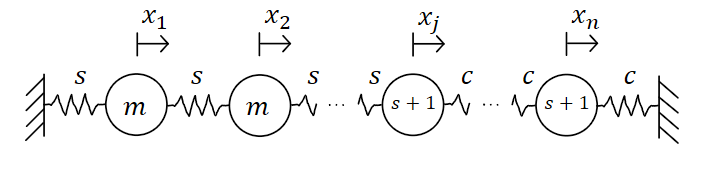
\includegraphics[width=0.9\textwidth, keepaspectratio]{./System1.png}
                  \caption{System 1}
                  \label{fig: System 1}
            \end{minipage}
            \hfill
            \begin{minipage}[ht]{0.49\linewidth}
                  \centering
                  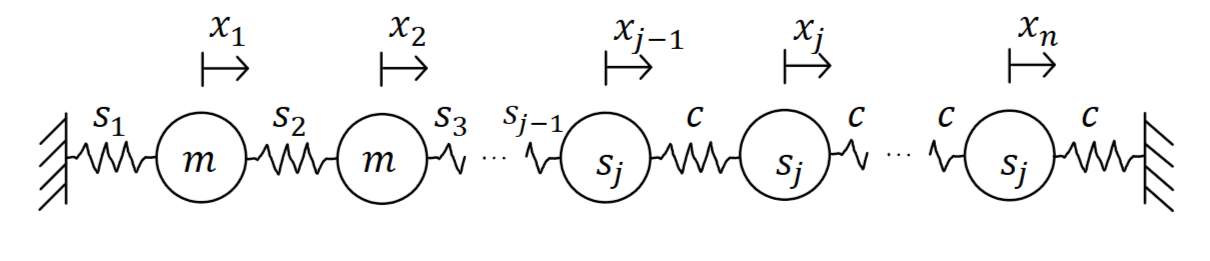
\includegraphics[width=0.9\textwidth, keepaspectratio]{./System2.png}
                  \caption{System 2}
                  \label{fig: System 2}
            \end{minipage}
      \end{figure}

      Der Vektor $x = (x_1,\dots,x_n)^T$ enthält hier die Auslenkungen der Massen aus ihrer Ruhelage und $s\in\R^l$ wird Design-Parameter (vgl. \cite[S. 2]{hauptteilTkachuk}) genannt.

      Falls in dieser Arbeit je von \zitat{Systemen} die Rede ist, so sind damit diese Systeme, die in den Abbildungen \ref{fig: System 1} und \ref{fig: System 2} beschrieben wurden, gemeint.

      Die Systeme aus Abb. \ref{fig: System 1} und \ref{fig: System 2} werden \zitat{Schwingerketten}\cite[S. 236]{maschinendynamikDresig} genannt,
      da sie aus starren Massen und masselosen Federn bestehen, die linear miteinander verbunden sind.
      Es existiert zudem in diesen Systemen keine Dämpfung.
      
      Laut \cite[S. 362-365]{maschinendynamikDresig} könne man für diese Systeme die \zitat{Differentialgleichung der freien Schwingungen}\cite[S. 365]{maschinendynamikDresig}
      erhalten, wenn man für jede Masse ein Kräftegleichgewicht aufstellt.
% komisch
      Diese Differentialgleichung besitzt folgende Form:
      \begin{equation}
            \label{eqn: Dgl freie Schwingungen}
            Kx+M\ddot x = 0
      \end{equation}

      wobei $K$ die Steifigkeitsmatrix und $M$ die Massenmatrix des Systems sind.
      Da genau diese Matrizen benötigt werden, um die Eigenkreisfrequenzen zu berechnen, ist das Ziel dieses Kapitels die Systeme von Kräftegleichgewichten
      aufzustellen und anschließend so umzuformen, dass eine Gleichung der Form (\ref{eqn: Dgl freie Schwingungen}) entsteht.
      Anhand dieser Gleichung werden die Matrizen abgelesen.
% sehr komisch
      Dafür wird der erste Abschnitt die im System wirkenden Kräfte und die Anwendung des Prinzips von d'Alembert behandeln.
      Im zweiten Abschnitt werden die Matrizen der Systeme bestimmt und anschließend wird in Abschnitt \ref{sec: Formel EW}
      die Formel für die Berechnung der Eigenkreisfrequenzen hergeleitet und umgeformt. 
      
      \section{Herleitung durch das Prinzip von d'Alembert}
            Nach \cite{d_AlembertPrinzip} besage das Prinzip von d'Alembert, dass die Summe aller wirkenden Kräfte in einem beschleunigten System verschwinde.

            Wir betrachten hier ein beschleunigtes System, da man in den Systemen die Massen von einem festen Standpunkt beobachtet.
            Daher gibt es für jede Masse eine Auslenkung aus der Ruhelage\footnote{man könnte auch ein System betrachten,
            in dem die Auslenkung einer bestimmten Masse immer gleich Null ist, in diesem System würden alle anderen Auslenkungen von dieser einen abhängen.}.

            Somit wird zuerst ein Kräftegleichgewicht aufgestellt und anschließend in eine Gleichung über Matrizen umgeformt,
            wodurch man die Massen- und Steifigkeitsmatrix erhält.
% In Maschinendynamik war von Koeffizientenvgl die Rede, könnte man auch einbauen
% Es muss irgendwo eine Quelle geben, die genau das sagt
            Da diese Herleitung auf Kräftegleichgewichten beruht, werden nun die agierenden Kräfte kurz erläutert:

            Die Federkraft \FL wird laut \cite{federkraft} durch
            \begin{equation}
                  \label{eqn: Federkraft}
                  \FL = c\cdot s
            \end{equation}
            berechnet, wobei $c$ die Federkonstante und $s$ die Auslenkung der Feder aus der Ruhelage ist.

            Beachte, dass nach Definition die Federkraft entgegen der Auslenkung wirkt, da bei Auslenkung die Feder in die Ruhelage zurückkehren will.
                  
            Der Betrag $F_T$ der Trägheitskraft ist nach \cite{trägheitskraft} definiert durch:
            \begin{equation}
                  \label{eqn: Trägheitskraft}
                  F_T = m\cdot a
            \end{equation}
            mit Masse $m$ und Beschleunigungsvektor $a$.    
            
            Beachte, dass laut \cite{trägheitskraft} auch diese Kraft der Auslenkung entgegenwirkt.
            Für einen Kraftvektor \FT gilt daher:
            $$\FT = -m\cdot a$$

            Um das Schemas der Kräfte klarer zu gestalten, werden die Kraftpfeile immer so gezeichnet, dass ihre Werte nichtnegativ sind.
            Hier bedeutet das, dass beide Kräfte entgegen der Auslenkung gezeichnet werden, dies kann man auch in Abb. \ref{fig: KräfteAnFeder} erkennen.
% Schemas, Kraftschemas,...
            Beide Kräfte werden in Abb. \ref{fig: KräfteAnFeder} veranschaulicht.

            \begin{figure}[h!t]
                  \centering
                  \includegraphics[width=0.2\textwidth, keepaspectratio]{./Federkraft und Trägheitskraft.png}
                  \caption{wirkende Kräfte an einer Masse mit Feder, Ausschnitt aus \cite{BildKräfteFeder}}
                  \label{fig: KräfteAnFeder}
            \end{figure}
% in diesem ganzen Teil gibt es Verbesserungsbedarf
            In Abb. \ref{fig: KräfteAnFeder} ist $z$ die Auslenkung und demnach gilt $F_L = c\cdot z$ (vgl. \cite{federkraft}).

            Da in dieser Ausarbeitung nur Feder-Masse-Systeme behandelt werden, kann man $s$ und $a$ auf die Auslenkungen $(\xk)_k$ zurückführen:
            Im Allgemeinen wird hier $s$ durch $(x_{k+1}-\xk)$ und $a$, wie schon in Abb. \ref{fig: KräfteAnFeder}, durch die zweite Ableitung $\ddot \xk$ beschrieben.
% Man könnte es auch umschreiben
            Betrachte nun ein System mit 3 Massen, wie es in Abb. \ref{fig: 3 Massen System} dargestellt wird.
            Anhand dieses Systems soll eine allgemeines Kräftegleichgewicht aufgestellt werden.

            \begin{figure}[h!t]
                  \centering
                  \begin{minipage}[ht]{0.49\linewidth}
                        \centering
                        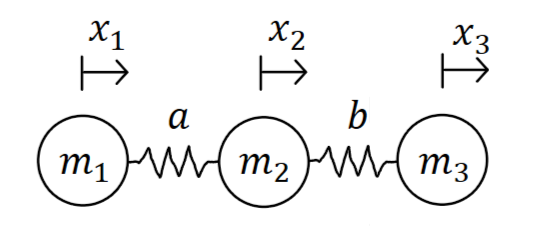
\includegraphics[width=0.7\textwidth, keepaspectratio]{./3 Massen System.png}
                        \caption{System mit 3 Massen}
                        \label{fig: 3 Massen System}
                  \end{minipage}
                  \hfill
                  \begin{minipage}[ht]{0.49\linewidth}
                        \centering
                        \includegraphics[width=0.7\textwidth, keepaspectratio]{./src/Kräfte Masse 1D.png}
                        \caption{Kräfte an frei geschnittener Masse}
                        \label{fig: Kräfte Masse 1D}
                  \end{minipage}
            \end{figure}

            Für $m_2$ erhält man die wirkenden Kräfte, wie sie in Abb. \ref{fig: Kräfte Masse 1D} dargestellt wurden.

            Beachte, dass die Kraftpfeile hier korrekt eingezeichnet wurden:
            Sei $x_1 \equiv x_3 \equiv 0$, dann folgt:
            $$x_2 > 0 \Rightarrow a(x_2-x_1) > 0 \Rightarrow \text{\zitat{Feder will sich zusammenziehen}}$$
            und analog
            $$x_2 < 0 \Rightarrow b(x_3-x_2) > 0 \Rightarrow \text{\zitat{Feder will sich zusammenziehen}}$$
            Mit dem Prinzip von d'Alembert führt dies auf die Gleichung
            \begin{equation}
                  \label{eqn: Gl für Masse}
                  m_2\,\ddot x_2 + a\,(x_2-x_1) - b\,(x_3-x_2) = 0
            \end{equation}

            Nehme man an,  es gelte $x_1 \equiv 0$\footnote{das entspricht in einer Differentialgleichung einer Dirichlet-Randbedingung},
            dann würde (\ref{eqn: Gl für Masse}) sich zu

            \begin{equation}
                  \label{eqn: Gl für Masse mit Rand links}
                  m_2\,\ddot x_2 + a\,x_2 - b\,(x_3-x_2) = m_2\,\ddot x_2 + (a+b)\,x_2 -b\,x_3 = 0
            \end{equation}
            reduzieren.

            In (\ref{eqn: Gl für Masse mit Rand links}) kann die Masse $m_1$ als unbeweglicher Rand betrachtet werden.
            Eine Gleichung dieser Form wird daher in den Systemen für den Punkt $k=1$ gelten.
            Analog kann mit $x_3\equiv 0$ verfahren werden, um für die Systeme aus den Abbildungen \ref{fig: System 1} und \ref{fig: System 2}
            eine Gleichung für den Punkt $k=n$ zu erhalten.

      \section{Ermittlung der Matrizen der Systeme}
            Nun werden die Massen- und Steifigkeitsmatrizen der Systeme bestimmt.
           
            Beginne dazu mit dem ersten System, siehe Abb. \ref{fig: System 1}.

            Die Form der Gleichung für die linke Masse ist durch (\ref{eqn: Gl für Masse mit Rand links}) gegeben.
            Für $k=2,\dots, n-1$ gilt eine Gleichung der Form (\ref{eqn: Gl für Masse}).
            
            Da die letzte Masse durch die rechte Feder mit dem Rand verbunden ist, gilt also $x_{n+1} \equiv 0$.
            Und analog zu (\ref{eqn: Gl für Masse mit Rand links}) erhält man
            $$(s+1)\,\ddot x_n + c\,(x_n-x_{n-1}) + c\,x_n = 0$$  

            Falls man nun alle Massen, Federkonstanten und Auslenkungen einsetzt, so erhält man nach Umstellen das Gleichungssystem

            $$\begin{cases}
                  m\ \ddot x_1 + 2s\,x_1 - s\,x_2 & = 0   \\
                  m\,\ddot x_k -s\,x_{k-1} + 2s\,x_k -s\,x_{k+1} & = 0,\quad k=2,\dots,j-1\\
                  (s+1)\,\ddot x_j -s\,x_{j-1} + (s+c)\,x_j -c\,x_{j+1} & = 0\\
                  (s+1)\,\ddot x_k -c\,x_{k-1} + 2c\,x_k -c\,x_{k+1} & = 0,\quad k=j+1,\dots,n-1\\
                  (s+1)\,\ddot x_n -c\,x_{n-1}+ 2c\,x_n & = 0
            \end{cases}$$


            Definiere nun $n$ und $j$ explizit, damit auch $M$ und $K$ explizit beschrieben werden können.
            \begin{equation}
                  \label{def: nUndJ explizit}
                  n=8,\\
                  j=n/2=4
            \end{equation}

            Dann kann das erste System zu einer Gleichung der Form (\ref{eqn: Dgl freie Schwingungen}) zusammengefasst werden.
            Hierbei gilt
            \begin{align}
                  M &= \diag(m, m, m, s+1, s+1,s+1, s+1,  s+1),\label{def: M1}\\
                  K &= \begin{pmatrix}
                        2s & -s &  &  &  &  &  &  \\
                        -s &  2s& -s &  &  &  &0  &  \\
                         & -s & 2s & -s &  &  &  &  \\
                         &  & -s & s+c & -c &  &  &  \\
                         &  &  & -c & 2c & -c &  &  \\
                         &  &  &  & -c & 2c & -c &  \\
                         & 0 &  &  &  & -c & 2c &  -c\\
                         &  &  &  &  &  & -c & 2c \\
                        \end{pmatrix}\label{def: K1}
            \end{align}\\

            Wende dieses Vorgehen auch für das System aus Abb. \ref{fig: System 2} an und erhalte
            
            $$\begin{cases}
                  m\ \ddot x_1 + (s_1+s_2)\,x_1 - s_2\,x_2 & = 0   \\
                  m\,\ddot x_k -s_k\,x_{k-1} + (s_k+s_{k+1})\,x_k -s_{k+1}\,x_{k+1} & = 0,\quad k=2,\dots,j-2\\
                  s_j\,\ddot x_{j-1} -s_{j-1}\,x_{j-2} + (s_{j-1}+c)\,x_{j-1} -c\,x_{j+1} & = 0\\
                  s_j\,\ddot x_k -c\,x_{k-1} + 2c\,x_k -c\,x_{k+1} & = 0,\quad k=j,\dots,n-1\\
                  s_j\,\ddot x_n -c\,x_{n-1}+ 2c\,x_n & = 0
            \end{cases}$$
            

            Dieses System kann man analog zu oben zu einer Gleichung der Form (\ref{eqn: Dgl freie Schwingungen}) umformen.
            Hier gilt nun aber, mit $n$ und $j$ wie in (\ref{def: nUndJ explizit})
            \begin{align}
                  M &= \diag(m, m, s_4, s_4, s_4, s_4, s_4, s_4)\label{def: M2}\\
                  K &= \begin{pmatrix}
                        s_1+s_2 & -s_2 &  &  &  &  &  &  \\
                        -s_2 &  s_2+s_3& -s_3 &  &  &  &0  &  \\
                              & -s_3 & s_3+c & -c &  &  &  &  \\
                              &  & -c & 2c & -c &  &  &  \\
                              &  &  & -c & 2c & -c &  &  \\
                              &  &  &  & -c & 2c & -c &  \\
                              & 0 & &  &  & -c & 2c &  -c\\
                              &  &  &  &  &  & -c & 2c \\
                        \end{pmatrix}\label{def: K2}
            \end{align}
                  
            Man beachte, dass für positiven Design-Parameter \s, bzw. für ein \s, wo alle Einträge positiv sind, die Massenmatrix regulär ist.

      \section{Zusammenhang Eigenwert und Eigenfrequenz}
            \label{sec: Formel EW}      
            Nach der Ermittlung der zugehörigen Matrizen bestimme nun die Formel für die Eigenkreisfrequenzen eines Systems.

            Die Schritte in diesem Abschnitt folgen \cite[S. 380]{maschinendynamikDresig} und \cite[S. 2]{hauptteilTkachuk}.
            Nach \cite[S. 380]{maschinendynamikDresig} gelte für die Auslenkungen der Massen mit $x$ statt $q$:
            $$x(t) = v\,\exp(i\w t),\ \ \ddot x(t) = -\w^2\,v \exp(i\w t)$$
            mit $v=(v_1,\dots,v_n)^T$ Vektor der Amplituden und der \zitat{noch unbekannten Eigenkreisfrequenz \w}\cite[S. 380]{maschinendynamikDresig}
            
            Diesen Ansatz wird in (\ref{eqn: Dgl freie Schwingungen}) eingesetzt und durch Division mit
            $\exp(i\w t)\footnote{offensichtlich ist die Division wohldefiniert, da $\exp(i\w t)\ne 0\ \forall \w, t\in\R,$}$ folgt:
            
            \begin{equation}
                  \label{eqn: allg EW Problem mit w}
                  (K-\w^2\,M)\,v = 0
            \end{equation}

            Die Gleichung kann ebenfalls in \cite[S. 380]{maschinendynamikDresig} gefunden werden.

            Man will diese Gleichung für $v\ne 0$ lösen, da man sonst eine triviale Lösung erhält, in der keine Masse schwingt.

            Um die Theorie aus Kapitel \ref{sec: EW Problem_Futamura} anzuwenden, so definiere
            $$\lambda_i := \w_i^2,\quad i=1,\dots,n$$

            Es folgt das allgemeine Eigenwertproblem
            \begin{equation}
                  \label{eqn: allg EW Problem mit lam}
                  (\K-\lambda\,\M)\,v = 0
            \end{equation}

            Man beachte, dass diese Gleichung genau die Form aus (\ref{eqn: allg EW Problem}) besitzt.
            Man kann für die vorgestellten Systeme folgern, dass für $N$ aus Kapitel \ref{sec: Futamura}
            $$N=\{1,\dots,n\}$$

            gilt, da die Massenmatrizen aus (\ref{def: M1}) und (\ref{def: M2}) Diagonalmatrizen mit positiven Einträgen auf der Diagonalen sind.
            Die Eigenwerte der Massenmatrix sind daher ebenfalls positiv.

            Für reguläre Massenmatrizen gelte nach \cite[S. 376]{matrixGolub} für (\ref{eqn: allg EW Problem mit lam}):
            $$(K-\lambda\,M)\,v = 0 \Leftrightarrow (M\inv K-\lambda\In)\,v=0$$
            und folglich
            \begin{equation}
                  \label{eqn: Ew Pencil gleich Ew Matrix}
                  \lambda(K, M) =\lambda(M\inv K,\In) = \lambda(M\inv K)
            \end{equation}

            Somit sind die Eigenwerte des Matrix-Pencils $K-\lambda M$ und der Matrix $M\inv K$ gleich.

            Da auch $M\inv$ eine Diagonalmatrix ist, so ist $M\inv K$ für die vorgestellten Systeme symmetrisch.
            Es gilt daher für die Systeme aus Abb. \ref{fig: System 1} und \ref{fig: System 2}
            \begin{equation}
                  \label{eqn: alle Ew reell}
                  \lambda(K, M) = \lambda(M\inv K) \subset \R
            \end{equation}
            wobei \cite[S. 393]{matrixGolub} angewendet wurde.

            Durch Bemerkung \ref{bem: B reg impl pencil reg} folgt ferner, dass die Matrix-Pencil der Systeme regulär sind.

\chapter{Zählung von Eigenwerten}
\label{sec: EW Zählung}
% vielleicht eher Finden der Zielfunktion nennen
      Nun wende man sich dem Finden einer Zielfunktion zu, die die Anzahl der Eigenwerte auf einem Intervall beschreibt.
      Diese gesuchte Funktion soll von dem Design-Parameter $s$ (vgl. \cite[S. 2]{hauptteilTkachuk}) ab und wird offenbar minimal,
      wenn kein Eigenwert des Matrix-Pencils in dem Intervall liegt.

      \section{Vorüberlegungen}
            Die in diesem Abschnitt erwähnten Schritte stammen aus \cite[S. 2-4]{hauptteilTkachuk}.

            Betrachte Gleichung (\ref{eqn: allg EW Problem mit lam}), durch die Definition $\lam = \w^2$ verändert sich auch das Intervall, welches man betrachtet:
            $$\lamAlamB:=\wAwB$$
% \w_a und \w_b nicht erklärt
            Definiere nun die Funktion $h$ wie folgt:
            $$h(\lambda):=\1_{[\lambda_a,\lambda_b]}(\lambda)$$

            Da man nur daran interessiert ist, ob ein Eigenwert in dem Intervall liegt oder nicht, definiere

            $$\mu := \sum_{j\in N} h(\lambda_j)$$

            Nach Kapitel \ref{sec: Formel EW} gilt aber $N=\{1,\dots,n\}$.\\
            Obwohl diese Funktion die Anzahl der Eigenwerte korrekt beschreibt, gibt es einige Schwachstellen, sollte man diese Funktion minimieren wollen:
            Die Funktion ist eine Treppenfunktion, damit ist sie nicht stetig und alle Ableitungen sind gleich 0, also unbrauchbar für Minimierungsalogrithmen, die eine Ableitung verwenden.

            Diese Probleme kann man teilweise umgehen, indem man die Funktion auf dem Intervall $[\lambda_a, \lambda_b]$ gewichtet.

            Um die Eigenwerte effektiv aus dem Intervall zu entfernen, nutze eine Gewichtungsfunktion, die auf dem ganzen Intervall positiv und konkav ist (vgl. \cite[S. 3]{hauptteilTkachuk}).
            Diese Funktion sorgt dafür, dass Eigenwerte in der Mitte des Intervalls stärker ins Gewicht fallen
            und somit die Eigenwerte zuerst aus der Mitte des Intervalls zum Rand gehen und ihn anschließend überqueren.
            Nach \cite[S. 3]{hauptteilTkachuk} sei die Funktion
            $$g(z) = -(z-((1+\alpha)\lambda_a -\alpha\lambda_b))(z-((1+\alpha)\lambda_b-\alpha\lambda_a))$$
            sehr geeignet, man könnte aber auch andere Funktionen definieren, die diese Eigenschaften besitzen.
            In den Funktionen stellt $\alpha>0$ einen Parameter dar, der dafür sorgt, dass die Funktion auf \lamAlamB positiv ist.
            $\alpha$ wird Inflationsparameter (vgl. \cite[S. 3]{hauptteilTkachuk}) genannt.
% Inflationsparameter

            Man findet so die erste Funktion, welche man mit Verfahren der Optimierung sinnvoll minimieren könnte:
            \begin{equation}
                  \label{def: J original}
                  J(s) = \sum_{j=1}^n g(\lambda_j)h(\lambda_j)
            \end{equation}

            Für diese Formel benötigt man allerdings alle Eigenwerte, diese müssten vorher berechnet werden.
            Auch hängen weder $g$ noch $h$ explizit von $s$ ab, daher kann die Funktion \J in dieser Form zwar zur gewichteten Zählung der Eigenwerte benutzt werden,
            aber nur über Umwege gibt diese Funktion an, in welche Richtung man gehen sollte, um die gewichtete Eigenwertzählung schnellstmöglich zu minimieren.
            
            Das Ziel ist daher eine Funktion, die explizit von \s abhängt, aber trotzdem die Eigenwerte gewichtet zählt.
            Dazu wird die Identität von Futamura aus Theorem \ref{thrm: IdentitätFutamura} benutzt.

            Betrachte also wie in Theorem \ref{thrm: IdentitätFutamura} eine Funktion, deren Polstellen die Eigenwerte sind.

            Die Funktion sei durch
            \begin{equation}
                  \label{eqn: ZielfunktionMitPolstellen}
                  L(z, s) = g(z)\sum_{j\in N} \frac{1}{z-\lam_j} = \sum_{j=1}^n \frac{g(z)}{z-\lam_j}
            \end{equation}

            definiert, ein Kurvenintegral über diese Funktion sei
            \begin{equation}
                  \label{eqn: IntZielfunktionMitPolstellen}
                  \frac{1}{2\pi i}\int_\gamma L(z, s)\ dz
            \end{equation}

            Um den Residuensatz sinnvoll anwenden zu können, muss die Kurve \gamm das Intervall \lamAlamB einschließen.
            Da aber alle Eigenwerte reell sind, so ist für $\gamma$ ein Kreis, welcher durch die Punkte $\lam_a$ und $\lam_b$ geht, optimal\footnote{dadurch wird sichergestellt,
            dass kein Eigenwert, der außerhalb des Intervalls \lamAlamB liegt, mit in die Zählung eingeht}.

            Allerdings muss zunächst gezeigt werden, dass diese Gleichung tatsächlich die Eigenwerte in dem Intervall gewichtet zählt, dafür benötigt man den Residuensatz,
            welcher im nächsten Abschnitt vorgestellt und angewendet wird.

      \section{Der Residuensatz und dessen Anwendung}
            Dieses Kapitel behandelt ausschließlich den Residuensatz und die Argumente, warum er auf (\ref{eqn: IntZielfunktionMitPolstellen}) anwendbar ist.
            Obwohl $L$ durch die Verteilung der Eigenwerte auch von dem Design-Parameter $s$ abhängt, vernachlässige diese Abhängigkeit in diesem Abschnitt.

            \begin{theorem}(Theorem 9.2 (Residue theorem)\cite[S. 141]{complexAnalysis})\\
                  \label{thrm: Residuensatz}
                  Sei $f$ analytisch auf $\Omega$, mit Ausnahme der isolierten Singularitäten $a_1,\dots,a_n$. Wenn für einen Kreis $\gamma\subseteq\C$
                  die Bedingungen $\gamma \sim 0$ und $a_j\notin \gamma,\ j=1,\dots,n$ erfüllt sind, dann
                  $$\int_\gamma f(z)\ dz = 2\pi i\sum_{k=1}^{n} n(\gamma, a_k)\Res_{a_k}f$$
            \end{theorem}
            Beweis: siehe \cite[S. 142]{complexAnalysis}

            Die folgenden Aussagen erklären die Voraussetzungen und das Resultat des Theorems und stammen aus \cite{complexAnalysis}.
            Die Aussagen und Definitionen werden nur kurz angeschnitten, da man sie in dieser Ausarbeitung nur für den Residuensatz (Theorem \ref{thrm: Residuensatz})
            und Gleichung (\ref{eqn: IntZielfunktionMitPolstellen}) verwendet. Die Beweise sind ebenfalls dort wiederzufinden.
            \begin{itemize}
% nicht alle sind fett markiert
                  \item \textbf{analytisch in }$\mathbf{z:}$ ist eine Eigenschaft von komplexen Funktionen, die besagt, dass man die Funktion als eine Potenzreihe um $z$ entwickeln kann.
                        Für $L(z, s)$ reicht aber folgende Aussage (vgl. \cite[S. 24]{complexAnalysis}):
% man müsste die Funktion referenzieren
                        Für Polynome $p(z)$ und $q(z)$ sei die rationale Funktion $L(z):=\frac{p(z)}{q(z)}$ analytisch auf $\{z\in\C: q(z)\ne 0\}$.
                        
                        Offenbar ist $L(z)$ eine rationale Funktion:

                        $$L(z) = \frac{p(z)}{q(z)}$$
                        mit 
                        \begin{align*}
                              p(z) &= \sum_{j=1}^{n}\prod_{\underset{i\ne j}{i=1}}^{n} z-\lambda_i,\\
                              q(z) &= \prod_{i=1}^{n} z-\lambda_i
                        \end{align*}

                        Offenbar sind $p$ und $q$ Polynome und $\{z: q(z)\ne 0\} = \C\setminus\{\lambda_i, i=1,\dots,n\}$
                        Daher ist $L$ analytisch auf $\C$ bis auf $\lambda_1,\dots,\lambda_n$
                  \item $\mathbf{b}$\textbf{ isolierte Singularität}:
                        Laut \cite[S. 74]{complexAnalysis} habe $L$ eine isolierte Singularität bei $\lambda_i$, wenn $L(\lambda_i)$ nicht definiert
                        und $L$ analytisch für $0<|z-\lambda_i|<\epsilon$ mit $\epsilon>0$ sei.

                        Offenbar ist $L(\lambda_i)$ nicht definiert für $i=1,\dots,n$ und da $L$ nur eine endliche Anzahl an Singularitäten besitzt, gilt:

                        \begin{equation}
                              \label{hilfe: complexAnalysis_isolierteSingularitäten}
                              L \text{ analytisch für } 0<|z-\lambda_i|<\widetilde{\epsilon},\quad i=1,\dots,n
                        \end{equation}
                        mit
                        $$\widetilde{\epsilon}:= \frac{1}{2}\,\min_{\underset{\lambda_i\ne \lambda_j}{i,j\in \{1,\dots,n\}} } |\lambda_i-\lambda_j|$$
% alternative: \min_{\lambda_i,\lambda_j\in\lambda(K,M): \lambda_i\ne\lambda_j}
                        Für den Fall, dass ein Eigenwert doppelt vorkommt, so ist der Eigenwert trotzdem eine isolierte Singularität,
                        da die Definition dies erlaubt.
% aus den Fingern gesaugt
                  \item $\mathbf{\frac{1}{2\pi i}\int_{\gamma} \frac 1 {z-a}\ dz:}$
                        Dieses Integral ist zwar nicht direkt für Theorem \ref{thrm: Residuensatz} von Bedeutung, allerdings wird es hier mehrmals benötigt.

                        Sei $z_0\in\C,\ r>0\text{ und }\gamma=\{z_0+r e^{it}: t\in [0,2\pi]\}$ (vgl. \cite[S. 48]{complexAnalysis}),
                        laut Proposition 4.13 aus \cite[S. 48]{complexAnalysis} gelte:
                        \begin{equation}
                              \label{hilfe: complexAnalysis_IntegralEinsDurchX}
                              \frac{1}{2\pi i}\int_\gamma \frac 1 {z-a}\ dz = \begin{cases}
                                    1 & \text{: } |a-z_0|<r \\
                                    0 & \text{: } |a-z_0|>r
                                    \end{cases}
                        \end{equation}
                  \item $\mathbf{n(\gamma, a)}$:
                        Sei $\gamma$ ein Kreis und $a\in \C\setminus \gamma$.
                        Nach Definition 5.4 aus \cite[S. 65]{complexAnalysis} ist die Windungsnummer $n(\gamma,a)$ von $\gamma$ über $a$ wie folgt definiert:
                        $$n(\gamma,a):= \frac{1}{2\pi i}\int_\gamma \frac{1}{\xi-a}\ d\xi$$

                        Man erkenne, dass mit (\ref{hilfe: complexAnalysis_IntegralEinsDurchX}) gilt:
                        \begin{equation}
                              \label{hilfe: complexAnalysis_WindungNullEins}
                              n(\gamma,a) = \begin{cases}
                                    1& \text{ : }a\in B_r(z_0)\\
                                    0& \text{ : }a\notin\overline {B_r(z_0)}
                              \end{cases}
                        \end{equation}
                        Hierbei benötigt man das $\gamma$ aus (\ref{hilfe: complexAnalysis_IntegralEinsDurchX}),
                        damit der Kreis in positive Richtung durchlaufen wird und kein Punkt (bis auf $z=z_0+r$) mehrmals vorkommt.
                  \item $\mathbf{\gamma \sim 0}$:
                        Durch Anwenden von Definition 5.5 aus \cite[S. 67]{complexAnalysis} folgt:
                        $$\gamma \sim 0 \Leftrightarrow n(\gamma, a)=0\ \forall a\notin \C$$
% aber hier ist nicht wirklich Omega gleich \C, es gibt ja noch die Polstellen
                        Offenbar gilt für alle $\alpha \in \C^C$
                        $$n(\gamma, \alpha) = 0$$

                  \item $\mathbf{\Res_af}$:
                        Nach Beispiel 9.3 aus \cite[S. 142]{complexAnalysis} gilt für eine einfache Polstelle:
                        \begin{equation}
                              \label{hilfe: complexAnalysis_Residuum}
                              \Res_af = \lim_{z\to a} (z-a)f(z)
                        \end{equation}
                        Anwenden auf $\Res_{\lambda_i}L$ ergibt:
                        \begin{align*}
                              \Res_{\lambda_i}L =& \lim_{z\to \lambda_i} \sum_{j=1}^{n} (z-\lambda_i)\frac{g(z)}{z-\lambda_j}
                              = g(z)\underbrace{\sum_{\underset{j\ne i}{j=1}}^{n} \frac{z-\lambda_i}{z-\lambda_j}}_{\to 0} + g(z)\frac{z-\lambda_i}{z-\lambda_i} \\
                              =& g(\lambda_i)
                        \end{align*}

                        Für ein beliebiges $\widetilde \lambda \in \C$\footnote{falls $\widetilde{\lambda}$ keiner der Eigenwerte ist,
                        dann gilt offenbar $P_{\widetilde \lambda} = \varnothing$} sei
                        $$P_{\widetilde \lambda} :=\{i\in\{1,\dots,n\}: \lambda_i = \widetilde{\lam}\}$$

                        Dann gilt:
                        \begin{align*}
                              L(z) =& \sum_{i=1}^{n} \frac{g(z)}{z-\lam_i}
                              = \sum_{i\in P_{\widetilde \lambda}} \frac{g(z)}{z-\widetilde{\lambda}}+\sum_{N^C\cap\{1,\dots,n\}}\frac{g(z)}{z-\lam_i}\\
                              =& \frac{|P_{\widetilde \lambda}| g(z)}{z-\widetilde{\lambda}}+\sum_{N^C\cap\{1,\dots,n\}}\frac{g(z)}{z-\lam_i}
                        \end{align*}

                        Und für $\Res_{\widetilde{\lam}}L(z)$ folgt:
                        $$\Res_{\widetilde{\lam}}L(z) = |P_{\widetilde \lambda}|\ g(\widetilde{\lam})$$
% ist vllt alles unnütz gewesen
                        Für mehrfach vorkommende Eigenwerte entstehen somit keine Änderungen. 
            \end{itemize}

            Damit wurde gezeigt, dass der Residuensatz auf die Funktion $L$ angewendet werden kann.

            Mit dem Residuensatz (Theorem \ref{thrm: Residuensatz}) gilt folglich für (\ref{eqn: IntZielfunktionMitPolstellen}):
            $$\frac 1 {2\pi i}\int_\gamma L(z,s)\ dz = \sum_{k=1}^{n} n(\gamma, \lambda_k) \Res_{\lambda_k}L = \sum_{k=1}^{n} n(\gamma, \lambda_k) g(\lambda_k)$$

            mit \begin{align}
                  \gamma =& \{\Tilde{z_0} + \Tilde r\exp(i t): t\in [0,2\pi]\},\label{def: gamma}\\
                  \Tilde{z_0} =& \frac {\lambda_a+\lambda_b} {2},\quad\Tilde r = \frac {\lambda_b-\lambda_a} {2}\nonumber
            \end{align}

            Mit (\ref{hilfe: complexAnalysis_WindungNullEins}) folgt für $n(\gamma, \lam_k)$:
            $$n(\gamma, \lam_k) = \begin{cases}
                  1& \text{ : }\lam_k\in B_{\Tilde{r}}(\Tilde{z_0})\\
                  0& \text{ : }\lam_k\notin\overline {B_{\Tilde{r}}(\Tilde{z_0})}
            \end{cases}$$
            
            Da aber $\lam_k\in \R\ \forall k=1,\dots,n$, ist diese Gleichung äquivalent zu
            $$n(\gamma, \lam_k) = \begin{cases}
                  1& \text{ : }\lam_k\in (\lam_a,\lam_b)\\
                  0& \text{ : }\lam_k\notin \lamAlamB
            \end{cases} = \1_{\lamAlamB}(\lambda_k) = h(\lambda_k)$$

            Beachte, dass für den Fall $\lam_k \in \{\lam_a, \lam_b\}$ diese Theorie und auch der Residuensatz aus Theorem \ref{thrm: Residuensatz}
            keine Aussage trifft, dieser Fall tritt aber fast sicher nicht ein.

            Für (\ref{eqn: IntZielfunktionMitPolstellen}) folgt
            $$\frac 1 {2\pi i}\int_\gamma L(z,s)\ dz = \sum_{k=1}^{n} h(\lambda_k) g(\lambda_k) = J(s)$$

            Womit gezeigt wurde, dass tatsächlich (\ref{eqn: IntZielfunktionMitPolstellen}) die Eigenwerte auf dem Intervall gewichtet zählt.
% % kann auch rausgelassen werden
%             Ferner gelte nach \cite[S. 77]{complexAnalysisVL} der Residuensatz auch für \zitat{toy contours}\cite[S. 77]{complexAnalysisVL}.
% % Zitat überprüfen/ übersetzen
%             Beispiele für toy contours sind Rechtecke oder Kreisausschnitte (siehe \cite[S. 42]{complexAnalysisVL}).

      \section{Anwendung der Identität von Futamura und Differenzierung}
            
            Um nun die Abhängigkeit von \s zu offenbaren, nutze die Identität von Futamura (Theorem \ref{thrm: IdentitätFutamura}), wodurch folgt     
            \begin{align}
                  J(s) =&\, \frac 1 {2\pi i}\int_\gamma L(z,s)\ dz = \frac 1 {2\pi i}\int_\gamma g(z)\sum_{j\in N} \frac{1}{z-\lam_j}\ dz\nonumber\\
                  =&\, \frac 1 {2\pi i}\int_\gamma g(z)\tr((zM(s)-K(s))\inv M(s))\ dz\label{eqn: JGleichIntTr}
            \end{align}

            Diese Funktion hängt nun explizit von $s$ ab und kann daher in Kapitel \ref{sec: Programmieren} minimiert werden.
            
            Gehe zuletzt auf $\frac{\partial L(z,s)}{\partial s}$ ein, da diese Ableitung in Kapitel \ref{sec: Programmieren} benötigt wird.
            \begin{equation}
                  \label{eqn: AbleitungZielfunktion}
                  \frac{\partial L(z,s)}{\partial s} = g(z) \frac{\partial}{\partial s}\klammer{\tr(\underbrace{(zM-K)\inv M}_{=:B(z, s)})}
            \end{equation}

            und es gilt für $\frac{\partial}{\partial s} \klammer{\tr(B(z, s))}$:
            $$\frac{\partial}{\partial s} \klammer{\tr(B(z, s))} = \frac{\partial}{\partial s} \klammer{\sum_{i=1}^n (B(z, s))_{ii}}
            = \sum_{i=1}^n \frac{\partial}{\partial s} (B(z,s))_{ii} = \tr\klammer{\frac{\partial}{\partial s} B(z,s)}$$
            
            Ferner gilt für $\frac{\partial}{\partial s} B(z, s)$:
            \begin{align*}
                  \frac{\partial}{\partial s} B(z, s) =& \frac{\partial D}{\partial s} \ M + D \ \frac{dM}{ds}\\
                  =& - D \frac{d}{ds}(zM-K) D + D \ \frac{dM}{ds}\\
                  =& D \ \frac{dM}{ds} - D \klammer{z \frac{dM}{ds}-\frac{dK}{ds}} D
            \end{align*}

            Wobei der Lesbarkeit halber $D:=(zM-K)\inv$ gilt und im 2. Schritt die Formel
            $$\nabla A(t)\inv = -A(t)\inv\ \nabla A(t)\ A(t)\inv$$
            angewendet wurde.\\
% man müsste eig d/ds_i betrachten
            Beweis: siehe \cite{derivativeInverseMatrix}\qed
% in Quelle wurde t auf ein Intervall beschränkt, A muss Inverse haben und stetig diffb. sein für alle t, das müsste man noch zeigen

            Die endgültige Formel für die Ableitung von $L$ ist
            \begin{equation}
                  \label{eqn: vollständigeAblL}
                  \frac{\partial L(z,s)}{\partial s} = g(z)\,\klammer{\tr\klammer{D \ \frac{dM}{ds}} - \tr\klammer{D \klammer{z \frac{dM}{ds}-\frac{dK}{ds}} D}}
            \end{equation}
% man könnte noch auf die Wohldefiniertheit eingehen, da es mit den Dimensionen passt, aber es geht erstmal
            

% ist hier nicht richtig, da B\in \Cnn
            % Beachte, dass für $s\in \R^l$, $z$ fest und $B\in \R^{n\times n}$ gilt:

            % $$B(z, \cdot): \R^l \to \R^{n\times n}\Rightarrow \frac{\partial}{\partial s} B(z, s) : \R^l\to \R^{n\times n}\times \R^l \Rightarrow \tr\klammer{\frac{\partial}{\partial s} B(z, s)}: \R^l \to \R^l$$

            % Man kann sich $\frac{\partial}{\partial s} B(z, s)$ als eine $n\times n$-Matrix vorstellen, in der jeder Eintrag ein Vektor in $\R^l$ ist.
            % Daher summiert man auch mit der Spur die Vektoren in $\R^l$ auf der Diagonalen auf und erhält selber wieder einen Vektor in $\R^l$.

\chapter{Implementierung}
\label{sec: Programmieren}

      Man wende sich nun der Implementierung des Minimierungsverfahrens zu.
      Wie schon in (\ref{def: nUndJ explizit}) erwähnt gilt für beide Systeme aus Kapitel \ref{sec: MS Matrizen}
      $$n=8,\quad j=4$$
      Es gibt aber noch mehr Parameter, die zuerst definiert werden müssen:
      \begin{itemize}
            \item für System 1 aus Abb. \ref{fig: System 1} gelte
            \begin{itemize}
                  \item $\lambda_a = 1.5$
                  \item $\lambda_b = 2.5$
                  \item $s_0 = 3.5\in\R$
                  \item $\Omega = [2,5]\subset \R$
                  \item $m = 4$
                  \item $c = 1.5$
            \end{itemize}
            \item für System 2 aus Abb. \ref{fig: System 2} gelte
            \begin{itemize}
                  \item $\lambda_a = 0.9$
                  \item $\lambda_b = 1.5$
                  \item $s_0 = (0.7, 0.7, 0.7, 1.5)^T\in \R^4$
                  \item $\Omega = [1,2]^3\times [0.5,3.5]\subset \R^4$
                  \item $m = 2$
                  \item $c = 0.75$
            \end{itemize}
      \end{itemize}

      Hierbei ist $\Omega$ die zulässige Menge des Design-Parameters $s$ und $s_0$ der Startwert der Minimierung.
      $m$ und $c$ wurden für die Massen- und Steifigkeitsmatrizen (\ref{def: M1}) - (\ref{def: K2}) verwendet.


      Es folgt zunächst noch der verwendete Algorithmus zur Minimierung und die Anwendung einer Quadraturformel
      zur Approximation des Integrals aus (\ref{eqn: JGleichIntTr}).
      \section{Theorie}
            Um die Funktion (\ref{eqn: JGleichIntTr}) zu minimieren, verwende eine Variation des Gradientenverfahrens
            aus \cite[S. 285]{optimierungBurkhard}, diese sei in Algorithmus \ref{alg: steilster Abstieg} beschrieben.
            \begin{algorithm}[h!t]
                  \caption{Verfahren des steilsten Abstiegs (vgl. \cite[S. 285]{optimierungBurkhard})}
                  \label{alg: steilster Abstieg}

                  \begin{algorithmic}
                        \Require $J(s), \nabla J(s)$
                        \Ensure $s^*$ mit $J(s^*)=0$
                        \State wähle $s\in \R^n;$
                        \Repeat
                              \State $d:=\nabla J(s);$
                              \State $s:=s-\lam_*d;$
                        \Until{$J(s)=0;$}
                        \State $s^*:=s;$
                        \Return $s^*;$
                  \end{algorithmic}
            \end{algorithm}

            Die Schrittweite $\lambda_*$ sei hier fest und da man das Minimum der gewichteten Eigenwertzählung bekannt ist,
            so benötigt man nur Information über $J(s)$, um ein Minimum zu erkennen.
            Diese Variation der Abbruchbedingung sorgt für eine schnellstmögliche Beendung des Minimierungsverfahrens.

            Allerdings werden für einen Schritt des Verfahrens $\nabla J(s)$ und $J(s)$ benötigt.
            Durch (\ref{eqn: Ew Pencil gleich Ew Matrix}) können zwar die Eigenwerte des Matrix-Pencils $K-\lambda M$ einfach bestimmt werden,
            aber die Ableitung kann dadurch nicht direkt ermittelt werden.

            Da keine Vorschrift zur Berechnung von $\nabla J(s)$ existiert, approximiere $J(s)$ zunächst durch eine Quadraturformel.

            Teile dazu $\gamma = \{\Tilde{z_0}+\Tilde r\exp(it): t\in [0,2\pi]\}$ in $m$ Teile auf:
            \begin{equation}
                  \label{def: gamma_k}
                  \gamma_k = \left\{\Tilde{z_0}+\Tilde r\exp(it): t\in \left[ 2\pi \frac k m, 2\pi \frac {k+1} m\right]\right\},\quad k=0,\dots,m-1
            \end{equation}

            Es folgt
            \begin{align}
                  \int_{\gamma_k} f(z)\ dz =& \int_{2 \pi \frac k m}^{2\pi \frac {k+1} m} f(\Tilde{z_0}+\Tilde r\exp(it))\,i\Tilde r\exp(it)\ dz\label{eqn: Teilintegral Kurve zu Intergral normal}\\
                  \approx& \frac{f(z_k)\,i\Tilde r\exp(\frac{2\pi i k}{m})+f(z_{k+1})\,i\Tilde r\exp(\frac{2\pi i (k+1)}{m})}{2} \frac{2\pi} m\nonumber\\
                  =& \klammer{f(z_k)+f(z_{k+1})\,\exp\klammer{\frac{2\pi i}{m}}}\frac{\pi i \Tilde r} m \,\exp(\frac{2\pi i k}{m})\nonumber
            \end{align}
            wobei $z_k:=\Tilde{z_0}+\Tilde r\exp\klammer{\frac {2\pi ik} m}, \quad k=0,\dots,m$.
            Es wurde hier eine Transformation zur Berechnung von Kurvenintegralen verwendet, siehe \cite[S. 21]{complexAnalysisVL}.
            Ferner wurde in der zweiten Zeile die Trapezregel angewendet, wie sie in \cite[S. 498]{numerikHermann} vorgestellt wird.
            
            Es gilt daher
            \begin{align}
                  J(s) =& \frac{1}{2\pi i}\sum_{k=0}^{m-1}\int_{\gamma_k} L(z,s)\ dz\nonumber\\
                  \approx& \frac{1}{2\pi i}\frac{\pi i \Tilde r} m\sum_{k=0}^{m-1}\left[\klammer{L(z_k, s)+
                  L(z_{k+1}, s)\,\exp\klammer{\frac{2\pi i}{m}}}\,\exp\klammer{\frac{2\pi i k}{m}}\right]\label{def: JSternTrapez}\\
                  =&:J_{\text{Tr}}^*(s)\nonumber
            \end{align}

            Der Index \zitat{Tr} steht hier für die verwendete Quadraturformel: die Trapezregel.
            In der Implementierung wird nur eine Funktion \zitat{JStern} definiert, diese kann aber jede beliebige Quadraturformel nutzen, um \J zu approximieren.
            Man kann leicht sehen, dass mit der Summen- und Faktorregel für Ableitungen
            $$\nabla J_{\text{Tr}}^*(s) = \frac{1}{2\pi i}\frac{\pi i \Tilde r} m\sum_{k=0}^{m-1}\left[\klammer{\partial_s L(z_k, s)+\partial_s L(z_{k+1}, s)\,
            \exp\klammer{\frac{2\pi i}{m}}}\,\exp\klammer{\frac{2\pi i k}{m}}\right]$$
            gilt.

            Die Faktoren vor $J^*(s)$ und $\nabla J^*(s)$ wurde nicht zusammengefasst, da in der Implementierung eine Funktion die Trapezregel auf eine Funktion anwendet,
            $\frac 1 {2\pi i}$ gehört aber nicht zur Quadraturformel dazu, sondern ist wegen der Anwendung des Residuensatzes vorhanden.

            Die Funktionen $\partial_s L(z, s)$ wurden schon in Kapitel \ref{sec: EW Zählung} in Gleichung (\ref{eqn: AbleitungZielfunktion}) definiert.

            Die Ableitungen $\frac{d M}{d s}$ und $\frac{d K}{d s}$ werden durch eine Differenz, wie sie in \cite[S. 16 f.]{numerikGrossmann} vorgestellt wird, approximiert.

            Wähle hier die Vorwärtsdifferenz
            \begin{equation}
                  \label{def: DiffVerfahren}
                  (D^+u)(x):=[u(x+h)-u(x)]/h
            \end{equation}
            mit $h=0.1$.

            Da im Allgemeinen $s\in \R^l$, werden hier aber partielle Ableitungen approximiert.
            Für die $i$-te partielle Ableitung gelte
            $$\frac{\partial M}{\partial s_i}\approx \frac{M(s+h e_i)-M(s)}{h}$$
            wobei $e_i$ der $i$-te Einheitsvektor ist.
 
      \section{Implementation}
            Die folgenden Programme wurden mit Python geschrieben. Hauptsächlich wird das Paket \zitat{numpy} genutzt, welches Berechnungen von Matrizen sehr vereinfacht.

            Bei Unwissenheit über einige Funktionen von Python wurden\linebreak
            \textit{https://numpy.org/doc/stable/} und \textit{https://stackoverflow.com/} verwendet.

            Die verschiedenen übergreifenden Funktionen, die von allen Programmen verwendet werden, findet man in \mbox{\cite[\textit{./Funktionen.py}]{github}}.

            In Kapitel \ref{sec: Programmieren} wird ausschließlich die Datei \mbox{\cite[\textit{./erste Implementierung.py}]{github}} behandelt.
            In dieser Datei werden sechs Durchläufe des Minimierungsverfahrens durchgeführt, beschrieben und die Plots gezeigt.
            Verbesserungen aus Kapitel \ref{sec: Verbesserungen} werden in den anderen Dateien zu finden sein.
            
            Falls bei einem Schritt des Minimierungsverfahrens $s$ die Menge $\Omega$ der zulässigen Werte verlässt,
            so wird der Design-Parameter mithilfe einer Projektion wie in \cite[S. 314]{optimierungJarreProjektion} wieder auf $\Omega$ abgebildet
            und im nächsten Schritt wird statt dem berechneten Wert die Projektion verwendet.
            
            Bei den Programmen gibt es eine Begrenzung für die Anzahl an Schritten pro Durchlauf der Minimierung.
            Falls ein Durchlauf mehr als 500 Schritte benötigen sollte, um zu einem Ergebnis zu kommen, wird er abgebrochen, damit ein einzelner Durchlauf nicht zu viel Zeit beansprucht.
            Diese Begrenzung kann man umgehen, indem man in Zeile 15 in \text{./erste Implementierung.py} den Wert des Arguments \mbox{\zitat{maxIter}} beliebig verändert.
            Man beachte aber, dass für nicht-positive Werte keine Begrenzung vorhanden ist.
            Das Verfahren wird in diesem Fall solange ausgeführt, bis es zu einem Ergebnis kommt, oder manuell abgebrochen wird.
            Diese Sperre wurde auf 10000 erhöht, um die Ergebnisse in Tabelle \ref{tab: Ergebnisse} zu erhalten.

            Es folgt nun eine Auflistung der 6 Durchläufe, die in diesem Programm durchgeführt werden.

            Es gehören immer 2 nacheinander folgende Durchläufe zusammen, da sie sich nur in der Anzahl der verwendeten Teilintervalle $m$
            und somit der Genauigkeit der Quadraturformel unterscheiden.
            Auch unterscheiden sich diese Durchläufe in der Schrittweite des Gradientenverfahrens $\lam_*$.

            Beim Ausführen des Programms werden noch verschiedene andere Kennzahlen, wie der Endpunkt des Design-Parameters, ausgegeben,
            hier werden aber nur die Anzahl an benötigten Iterationen und die dafür benötigte Zeit betrachtet.
            Die Zeit misst nur die Zeit, die für die Minimierung benötigt wird.
            Aufarbeitungen, wie das anschließende Berechnen der Eigenwerte, werden hier nicht gemessen. \\

            \begin{table}[ht]
                  \centering
                  \begin{tabular}{lllcc}
                       System & $m$ & $\lambda_*$ & Iterationen & Zeit in s\\
                       \hline
                       1 & $100$ & $0.05$ & $>10000$ & $>584$ \\ 
                       1 & $150$ & $0.05$ & $>10000$ & $>830$ \\
                       \hline
                       1 & $100$ & $0.5$ & $>10000$ & $>561$ \\
                       1 & $150$ & $0.5$ & $15$ & $1.2$ \\
                       \hline
                       2 & $100$ & $0.05$ & $150$ & $15.2$ \\
                       2 & $150$ & $0.05$ & $>10000$ & $>1592$ \\
                       \hline
                  \end{tabular}\\
                  \captionof{table}{Kennzahlen der ersten Implementierung\label{tab: Ergebnisse}}
            \end{table}

            Man kann schon an Tabelle \ref{tab: Ergebnisse} erkennen, dass dieses Verfahren nur selten zum Erfolg führt.

            Außerdem sind Zeiten über 9 Minuten für ein System mit nur 8 Freiheitsgraden und einem skalarem Design-Parameter völlig unzureichend.

            Man bemerke aber, dass dieses Verfahren funktionieren kann, wie man an den Durchläufen 4 und 5 sieht.

      \section{Grafiken und Erklärung}
            Man gehe nun genauer auf die Verläufe der Eigenwertzählung und die Verläufe der Eigenwerte selbst ein.
            Betrachte zuerst die ersten beiden Durchläufe.
            Um die folgenden Ausführungen zu unterstützen, werden die folgenden zwei Abbildungen auf die Schritte 0 bis 200 begrenzt.
            Nach dem Schritt verändern sich in diesen beiden Durchläufen bis Schritt 10000 weder die Eigenwert-Zählungen noch die Verteilung der Eigenwerte wesentlich.

            Der obere Plot eines Durchlaufs zeigt, wie sich die gewichteten und die ungewichtete Eigenwertzählung veränderten.
            Der untere Plot zeigt jeweils das vorgegebene Intervall und die Verteilung der Eigenwerte.
            Oft werden nur Ausschnitte gezeigt, um die Eigenwerte innerhalb diese Intervalls deutlicher zu erkennen.
            Es ist daher möglich, dass nicht alle Eigenwerte abgebildet werden.
            Die kompletten Abbildungen kann man aber durch Ausführen des Programms \textit{erste Implementierung.py} erhalten.
            
            Für diese beiden Durchläufe beschränke man sich auf die Verteilung der Eigenwerte.
            \begin{figure}[h!t]
                  \centering
                  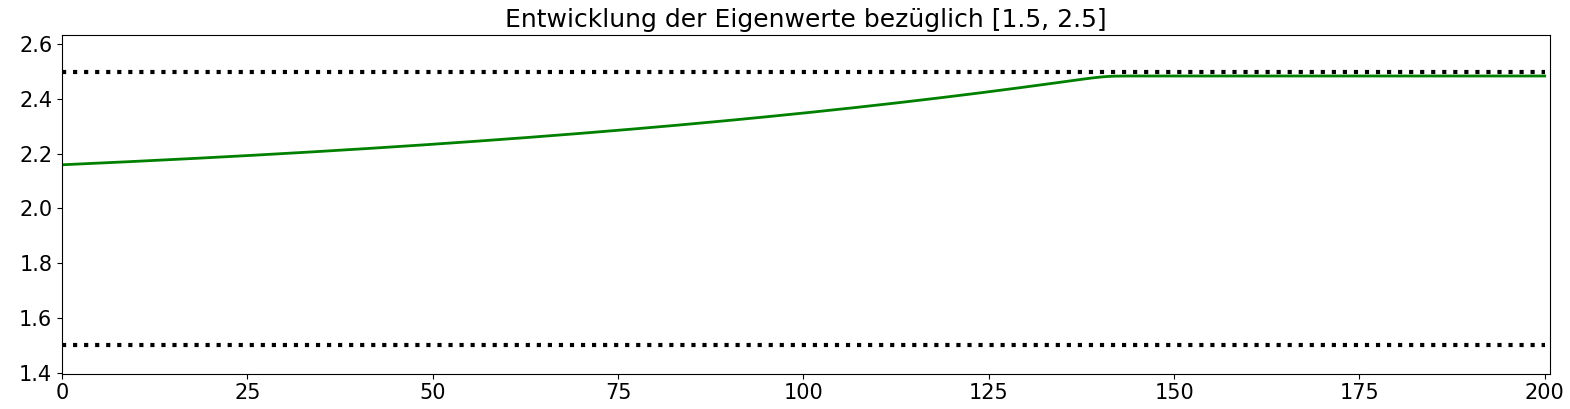
\includegraphics[width=0.9\textwidth, keepaspectratio]{./Original/Plot_1_100_0.05.png}
                  \caption{System 1, $m=100$, $\lambda_*=0.05$}
                  \label{fig: Plot_1_100_0.05}
            \end{figure}

            \begin{figure}[h!t]
                  \centering
                  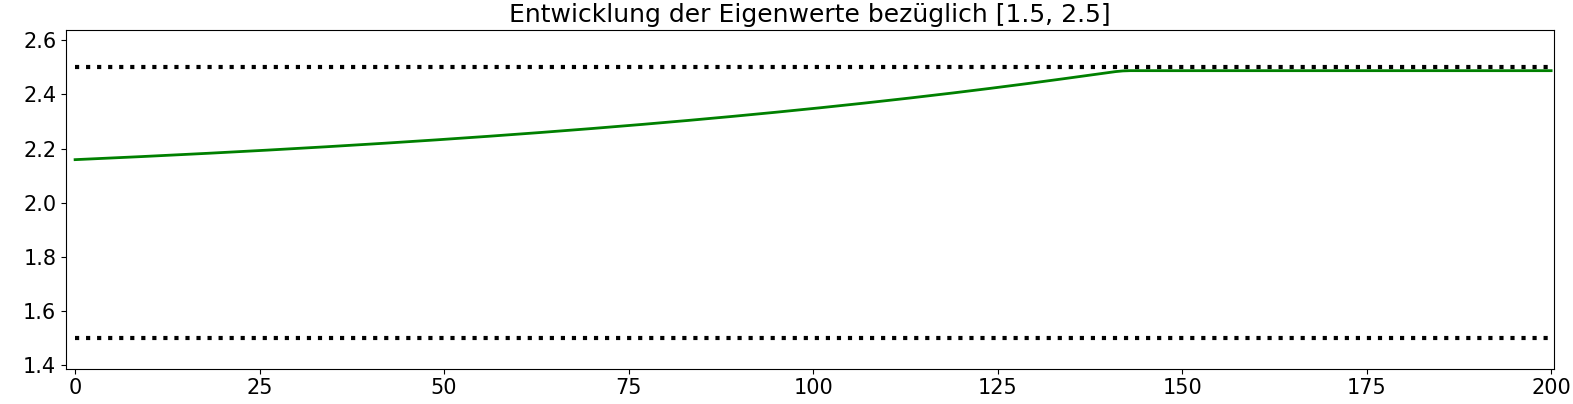
\includegraphics[width=0.9\textwidth, keepaspectratio]{./Original/Plot_1_150_0.05.png}
                  \caption{System 1, $m=150$, $\lambda_*=0.05$}
                  \label{fig: Plot_1_150_0.05}
            \end{figure}

            Die gepunkteten Linien stellen immer das Intervall \lamAlamB dar.
            Ferner werden die Eigenwerte in den Plots \zitat{Entwicklung der Eigenwerte} nicht mithilfe einer Legende beschriftet, da dies keinen Mehrwert bringt.
            Mit erster Eigenwert werde hier immer der größte Eigenwert bezeichnet, den man sehen kann, mit zweiter der nächstkleinere.
            Man sehe zuerst, dass sich der betrachtete Eigenwert dem oberen Rand des Intervalls ($\lam_b$) nähert, aber ihn nicht überschreitet.
            Daran ändert sich auch nach weiteren 9800 Schritten nichts, wie man in Tabelle \ref{tab: Ergebnisse} erkennen kann.
            Diese Durchläufe unterscheiden sich so minimal voneinander, dass die Unterschiede nur durch sehr starke Vergrößerung sichtbar werden.
            Dies kann man sich ebenfalls durch Ausführung des Programms klar machen.

            Bei den nächsten beiden Durchläufen betrachte nur die Schritte 0 bis 17. 

            \begin{figure}[h!t]
                  \centering
                  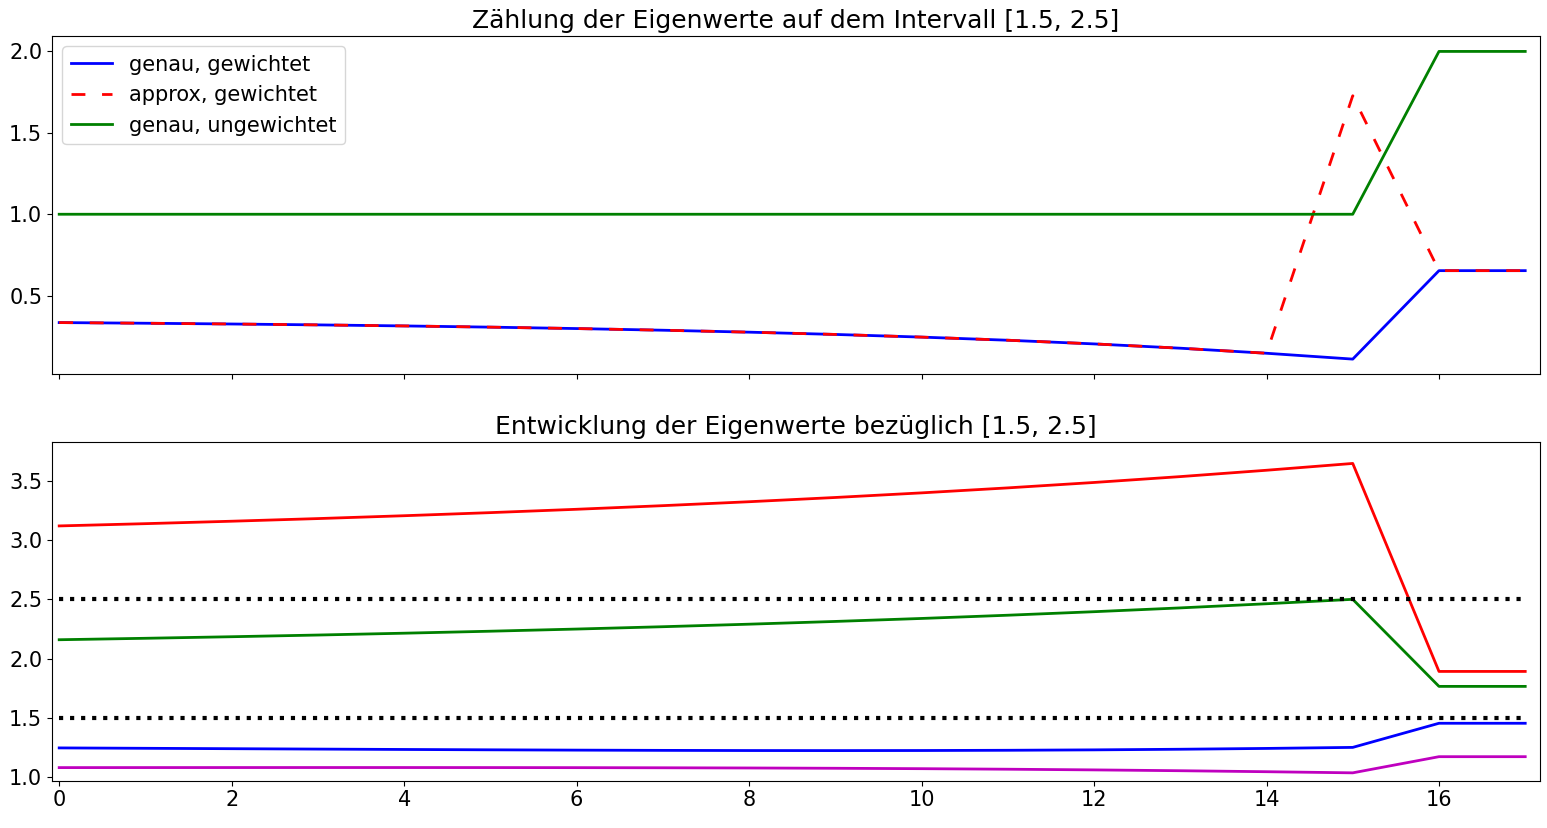
\includegraphics[width=0.9\textwidth, keepaspectratio]{./Original/Plot_1_100_0.5.png}
                  \caption{Plots zu System 1, $m=100$, $\lambda_*=0.5$}
                  \label{fig: Plot_1_100_0.5}
            \end{figure}

            \begin{figure}[h!t]
                  \centering
                  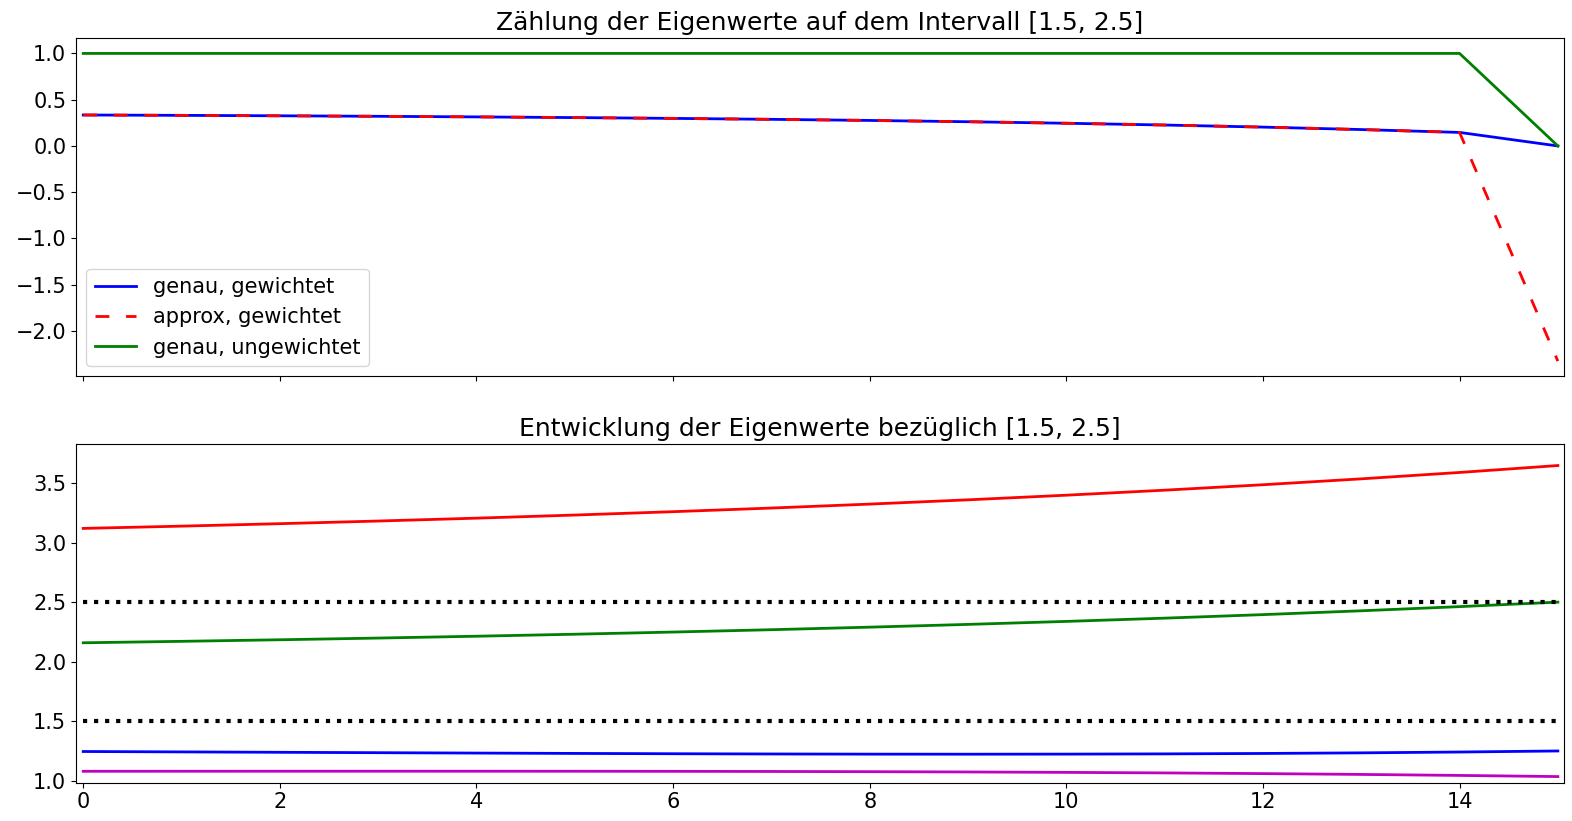
\includegraphics[width=0.9\textwidth, keepaspectratio]{./Original/Plot_1_150_0.5.png}
                  \caption{Plots zu System 1, $m=100$, $\lambda_*=0.5$}
                  \label{fig: Plot_1_150_0.5}
            \end{figure}

            Hier kann man die Unterschiede zwischen den Genauigkeiten der Quadraturformeln leicht erkennen: während in Abb. \ref{fig: Plot_1_100_0.5}
            nach Schritt 15 nicht alle Eigenwerte aus dem Intervall entfernt wurden, so befinden sich in Abb. \ref{fig: Plot_1_150_0.5} nach dem gleichen Schritt alle Eigenwerte außerhalb des Intervalls.
            Da die Abbruchbedingung des Gradientenverfahrens hier die genaue gewichtete Eigenwertzählung ist, wird das Gradientenverfahren nach diesem Schritt beendet.

            Man sehe aber auch, dass die approximierte gewichtete Eigenwertzählung bei beiden Durchläufen in Schritt 15 sehr stark von der genauen abweicht.
            Dies kann sehr wahrscheinlich auf die verwendete Quadraturformel zurückgeführt werden:
            Bei beiden Quadraturformeln wird L(z,s) an den Stellen $z=\lambda_a$ und $z=\lambda_b$ ausgewertet.
            Falls aber ein Eigenwert sich nahe des Intervallrands befindet, so befindet sich eine Stützstelle nahe einer Polstelle.
            Das führt zu unerwünschten Erscheinungen:
            In Abb. \ref{fig: Plot_1_100_0.5} wird die gewichtete Eigenwertzählung bei Schritt 15 viel zu hoch approximiert,
            in Abb. \ref{fig: Plot_1_150_0.5} wird sie bei Schritt 15 negativ.

            Bei Durchlauf \ref{fig: Plot_1_100_0.5} wird infolge dessen nicht mehr versucht, den zweiten Eigenwert zu vergrößern,
            damit er das obere Ende des Intervalls überschreitet, sondern der zweite Eigenwert wird so stark verringert, sodass nun sogar der erste Eigenwert im Intervall liegt.
            Obwohl die negative Approximation bei Abb. \ref{fig: Plot_1_150_0.5} einen Wert annimmt, der für die genauen Eigenwertzählung nicht möglich ist, so ändert es nichts an dem Verlauf,
            da in diesem Schritt alle Eigenwert außerhalb des Intervalls liegen und laut Algorithmus \ref{alg: steilster Abstieg}
            die genaue gewichtete Zählung verwendet wird, um zu entscheiden, ob ein Minimum erreicht wurde. Wie man sehen kann verschwinden die genauen Eigenwertzählung bei Schritt 15.
            Sollte man nur Informationen über die approximierte Zählung besitzen, so wäre das Verfahren, je nach Programmierung,
            nicht beendet worden, sondern fortgeführt worden, obwohl es ein Minimum erreicht hatte.

            Dieses Verhalten der approximierten gewichteten Eigenwertzählung wird in Kapitel \ref{sec: Verbesserungen} erneut angesprochen.

            Betrachte nun die Durchläufe von System 2.
            Es wurde sich auf die Schritte 0 bis 150 beschränkt, um diese im Detail sehen zu können.

            \begin{figure}[h!t]
                  \centering
                  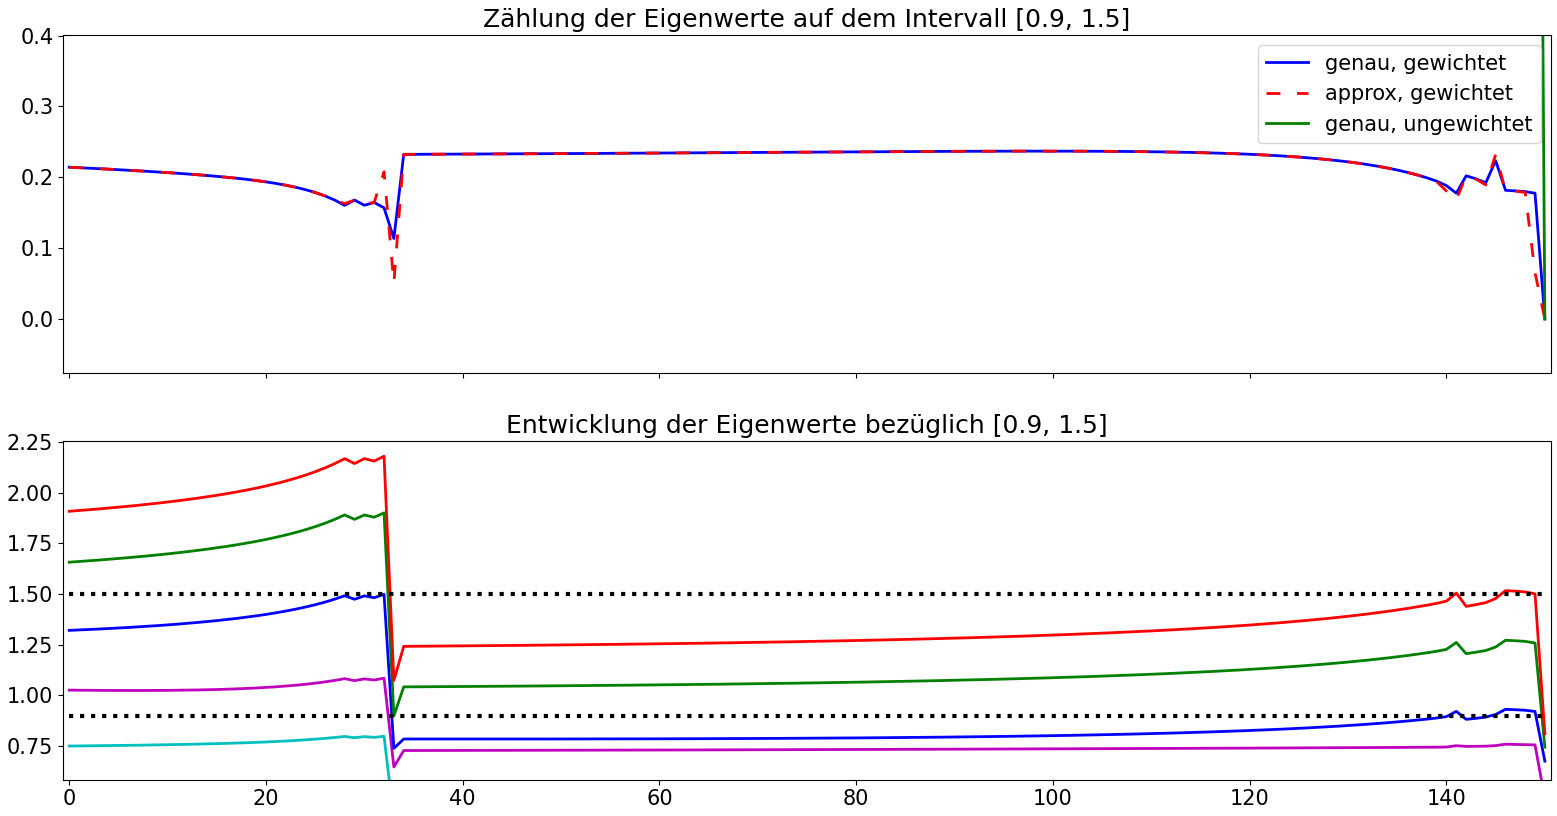
\includegraphics[width=0.9\textwidth, keepaspectratio]{./Original/Plot_2_100_0.05.png}
                  \caption{Plots zu System 2, $m=100$, $\lambda_*=0.05$}
                  \label{fig: Plot_2_100_0.05}
            \end{figure}

            \begin{figure}[h!t]
                  \centering
                  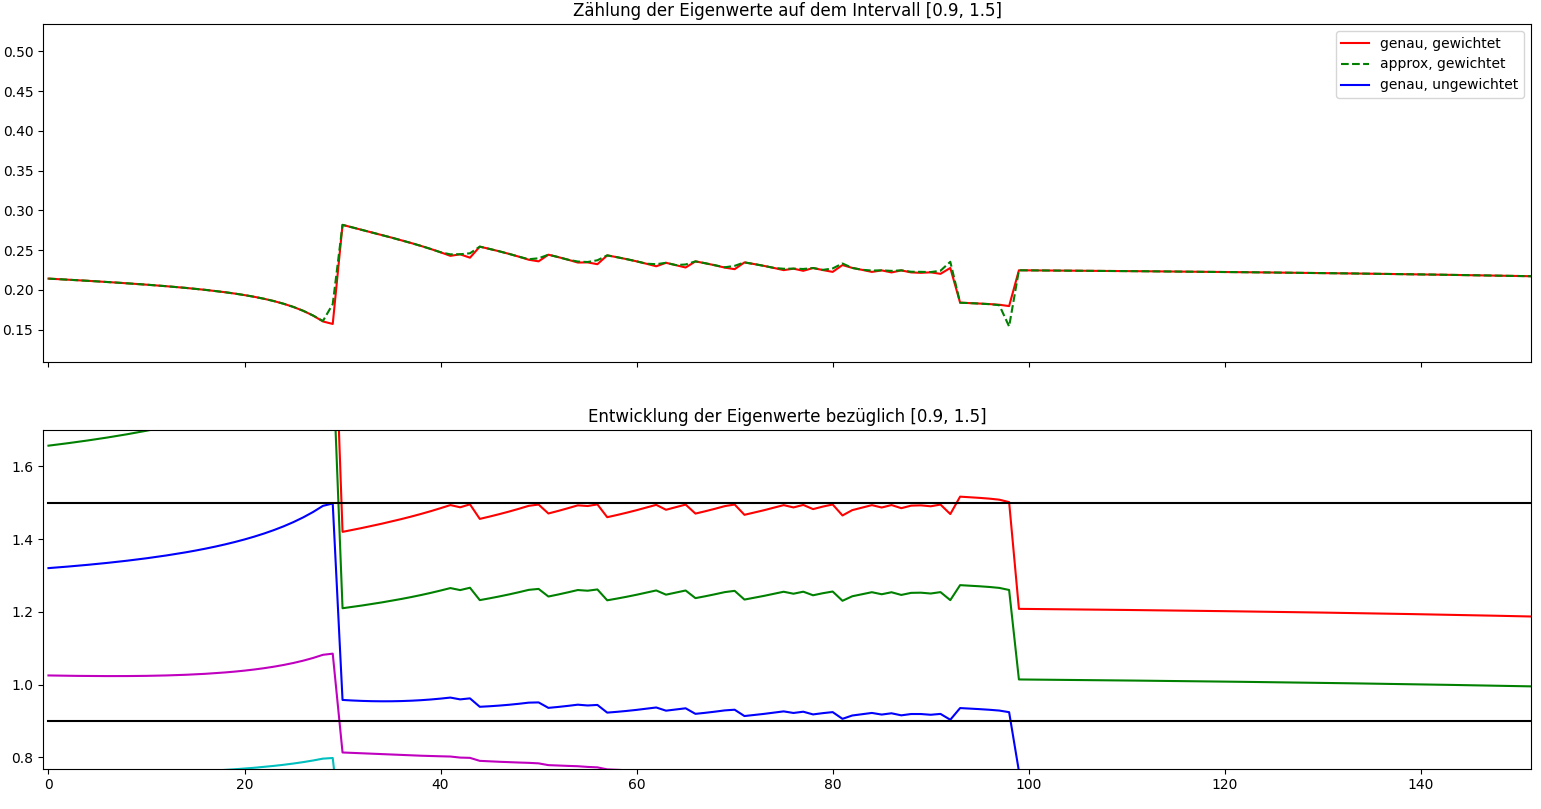
\includegraphics[width=0.9\textwidth, keepaspectratio]{./Original/Plot_2_150_0.05.png}
                  \caption{Plots zu System 2, $m=150$, $\lambda_*=0.05$}
                  \label{fig: Plot_2_150_0.05}
            \end{figure}

            Wie man leicht in Abb. \ref{fig: Plot_2_100_0.05} sehen kann, war das Erreichen eines Minimums nicht immer eine kontrollierte Veränderung:
            An beiden Stellen kam ein Eigenwert sehr nahe an eine der beiden Intervallgrenzen. Wie schon in den vorherigen Abbildungen führt das zu einer ungenauen Approximation der gewichteten Eigenwertzählung.
            Zufällig waren diese Ungenauigkeit und somit auch die Sprünge in Abb. \ref{fig: Plot_2_100_0.05} derart, dass nach dem zweiten Sprung alle Eigenwerte außerhalb des Intervalls lagen,
            wohingegen bei Abb. \ref{fig: Plot_2_150_0.05} die genauere Quadraturformel zur Folge hatte, dass nicht alle Eigenwerte nach diesen Sprüngen außerhalb des Intervalls lagen.

            Man könnte die Minimierung als instabiles System ansehen, da hier Veränderungen der Quadraturformel ausreichten, um den Verlauf der Eigenwerte komplett zu verändern\footnote{es reicht sogar ein Wechsel des Gerätes, welches das Programm ausführt, um unterschiedliche Ergebnisse hervorzubringen}.

\chapter{Verbesserungen}
\label{sec: Verbesserungen}
      In Kapitel \ref{sec: Programmieren} sind folgende Probleme deutlich zum Vorschein getreten:
      Einerseits ist die approximierte Zählung der Eigenwerte unzureichend, wenn sich ein Eigenwert in der Nähe der Intervallgrenzen befindet.
      Am einfachsten ist dies an den Abbildungen \ref{fig: Plot_1_100_0.5}, \ref{fig: Plot_1_150_0.5} und \ref{fig: Plot_2_100_0.05} zu sehen:
      Immer wenn ein Eigenwert in die Nähe der Intervallgrenze und damit der Integrationskurve kam,
      wurde die gewichtete Eigenwertzählung ungenau approximiert, was dazu führte, dass die Systeme in einem Schritt sehr große Sprünge ausführten.
      Auch das Verhalten des Eigenwerts in den Abbildungen \ref{fig: Plot_1_100_0.05} und \ref{fig: Plot_1_150_0.05} kann damit erklärt werden.
      Hier kam es zwar nicht zu Sprüngen, aber die Quadraturformel verhinderte, dass der Parameter \s genug verändert wird,
      sodass der Eigenwert das Intervall verlassen kann\footnote{die Tatsache, dass dieses Verhalten in der Quadraturformel begründet ist,
      kann in \mbox{\cite[\textit{./Verbesserung\_Trapez.py}]{github}} gesehen werden, dort wurden die Stützstellen der Trapezregel aus Kapitel \ref{sec: Programmieren} so verschoben, dass keine Stützstelle sich in der Nähe von $\lambda_a$ und $\lambda_b$ befindet}.
      Ferner sieht man anhand der Abbildungen \ref{fig: Plot_1_100_0.05}, \ref{fig: Plot_1_150_0.05} und \ref{fig: Plot_1_150_0.5},
      dass eine größere Schrittweite des Gradientenverfahrens deutlich bessere Ergebnisse hervorbringen kann.
      Allerdings ist eine zu hohe Schrittweite nicht immer von Vorteil, sollte sich ein Schritt des Verfahrens nahe an einer Lösung des Problems befinden.
      Man sehe zudem, dass sich viele der Durchläufe mit kurzen Schrittweiten $\lambda_*$ über lange Strecken kaum verändern.
      Um dem vorzubeugen berechne die Schrittweite des Gradientenverfahrens dynamisch, wie es auch im klassischen Gradientenverfahren \cite[S. 285 f.]{optimierungBurkhard} üblich ist.
      Zuletzt sind diese langen Zeiten für Probleme mit einstelligen Freiheitsgraden nicht wünschenswert,
      da einige tatsächlich verwendete Berechnungsmodelle $n>1.000.000$ Freiheitsgrade besitzen (vgl. \cite[S. 359]{maschinendynamikDresig}).

      \section{Verbesserte Quadraturformeln}
            Man wende sich zuerst der Verbesserung der Quadraturformel zu.
            Man erhofft sich hier, Ungenauigkeiten, die auftreten, wenn sich ein Eigenwert dem Intervallrand nähert, zu verringern, um große Sprünge in der Verteilung der Eigenwerte zu vermeiden.
            Durch verbesserte Quadraturformeln sollen die Eigenwerte das Intervall geordnet verlassen und nicht per Zufall/ während eines Schrittes wie in Abb. \ref{fig: Plot_2_100_0.05}.

            Man nutze daher eine Quadraturformel, welche das Integral zwar approximiert, aber nicht an den Stellen $\lambda_a$ und $\lam_b$ ausgewertet wird.

            Die einfachste Quadraturformel, die dies bewerkstelligt ist die \zitat{Mittelpunkts-Regel}\cite[S. 526]{numerikHermann}:

            Sei dazu $\gamma_k, k=0,\dots,m-1$ wie in (\ref{def: gamma_k}), nach (\ref{eqn: Teilintegral Kurve zu Intergral normal}) gilt:
            \begin{align*}
                  \int_{\gamma_k} L(z, s)\ dz =& \int_{2\pi \frac{k}{m}}^{2\pi\frac{k+1}{m}}L(\Tilde z_0+\Tilde r\exp(it), s)i\Tilde r \exp(it)\ dt\\
                  \approx& L(\Tilde z_0+\Tilde r\exp\klammer{\frac{2\pi i}{m}(k+\frac{1}{2})}, s)i\Tilde r \klammer{\frac{2\pi i}{m}(k+\frac{1}{2})} \frac{2\pi}{m}\\
                  =& L(z_{k+\frac{1}{2}}, s)(\Tilde z_0-z_{k+\frac{1}{2}}) \frac{2\pi i}{m}
            \end{align*}

            wobei die Definition $z_{k+\frac{1}{2}}:= \Tilde z_0+\Tilde r\exp(\frac{2\pi i}{m}(k+\frac{1}{2})), k=0,\dots,m$
            und die Formel der Mittelpunkts-Regel aus \cite[S. 526]{numerikHermann} verwendet wurde.

            Es gilt für $J(s)$:
            \begin{align}
                  J(s) =& \frac{1}{2\pi i}\sum_{k=0}^{m-1} \int_{\gamma_k} L(z, s)\ dz \approx \frac{1}{2\pi i}\sum_{k=0}^{m-1} L(z_{k+\frac{1}{2}}, s)(\Tilde z_0-z_{k+\frac{1}{2}}) \frac{2\pi i}{m}\nonumber\\
                  =&  \frac{1}{2\pi i}\left[\frac{2\pi i}{m}\sum_{k=0}^{m-1} L(z_{k+\frac{1}{2}}, s)(\Tilde z_0-z_{k+\frac{1}{2}})\right]=:J^*_{\text{Mittel}}(s)\label{def: JSternMittel}
            \end{align}

            Wobei wieder die Faktoren vor der Summe nicht gekürzt wurden, da der erste Faktor von der Anwendung des Residuensatzes stammt
            und der zweite Faktor ein Teil der Quadraturformel ist
            \footnote{falls man die Faktoren kürzen würde, erhält man die Stützstellen $z_k$ und Gewichte $\w_k$ aus \cite[S. 128]{grundlageFutamura},
            das Kürzen würde die Berechnung zwar beschleunigen, aber die Berechnung der $J^*$ wurde in \cite[\textit{./Funktionen.py}]{github} so implementiert, dass jede Quadraturformel genutzt werden kann}.

            Durch die Verwendung dieser Quadraturformel erhält man folgende Ergebnisse:

            \begin{table}[!ht]
                  \centering
                  \begin{tabular}{lllcc}
                       System & $m$ & $\lambda_*$ & Iterationen & Zeit in s\\
                       \hline
                       1 & $100$ & $0.05$ & $142$ & $3.7$ \\ 
                       1 & $150$ & $0.05$ & $143$ & $5.3$ \\
                       \hline
                       1 & $100$ & $0.5$ & $15$ & $0.5$ \\
                       1 & $150$ & $0.5$ & $15$ & $0.7$ \\
                       \hline
                       2 & $100$ & $0.05$ & $300$ & $13.9$ \\
                       2 & $150$ & $0.05$ & $289$ & $21.7$ \\
                       \hline
                  \end{tabular}\\
                  \captionof{table}{Kennzahlen bei Verwendung der Mittelpunkts-Regel}\label{tab: Ergebnisse_Mittelpunkt}
            \end{table}

            Die Ergebnisse und die zugehörigen Plots können auch in der Datei\linebreak
            \mbox{\cite[\textit{./Verbesserung\_Mittelpunkt.py}]{github}} betrachtet werden.

            Es fällt auf, dass die Minimierung in den ersten zwei Durchläufe im Vergleich zu den Durchläufen aus Tabelle \ref{tab: Ergebnisse} nun viel schneller erfolgen, da nur 142-143 Schritte benötigt werden.
            Natürlich wären diese Durchläufe auch schneller, wenn sie alle zu keinem Ergebnis kommen würden, da hier die Funktion pro Teilintervall nur an einer Stelle auszuwerten ist.

            Wie man ferner sehen kann, besteht in System 1 eine indirekte Proportionalität zwischen Schrittweite $\lambda_*$ und der Anzahl an Schritten, was auf die Eindimensionalität von Design-Parameter $s$ zurückzuführen ist.
            In den Durchläufen zu System 2 sieht man zudem, dass sich die Anzahl an Iterationen für $m=100$ im Vergleich zu Tabelle \ref{tab: Ergebnisse} verdoppelt,
            allerdings ist dies auf die Tatsache zurückzuführen, dass der Verlauf der Eigenwerte keine plötzlichen Sprünge mehr ausführt, wie sie in Abb. \ref{fig: Plot_2_100_0.05} zu sehen waren.

            Zuletzt sei angemerkt, dass sich die Zeiten zwischen 2 Durchläufen mit unterschiedlicher Anzahl an Teilintervallen $m$ ungefähr im Verhältnis $1:1,5$ befinden.

            Die folgende Abbildung zeigt, wie sich die Eigenwerte des ersten Durchlaufs verändern. Da ab nun alle Plots von System 1 sehr ähnlich zueinander sind,
            sei Abb. \ref{fig: Plot_1_100_0.05_Mittelpunkt} in diesem Abschnitt der einzige Plot zu System 1.

            \begin{figure}[ht]
                  \centering
                  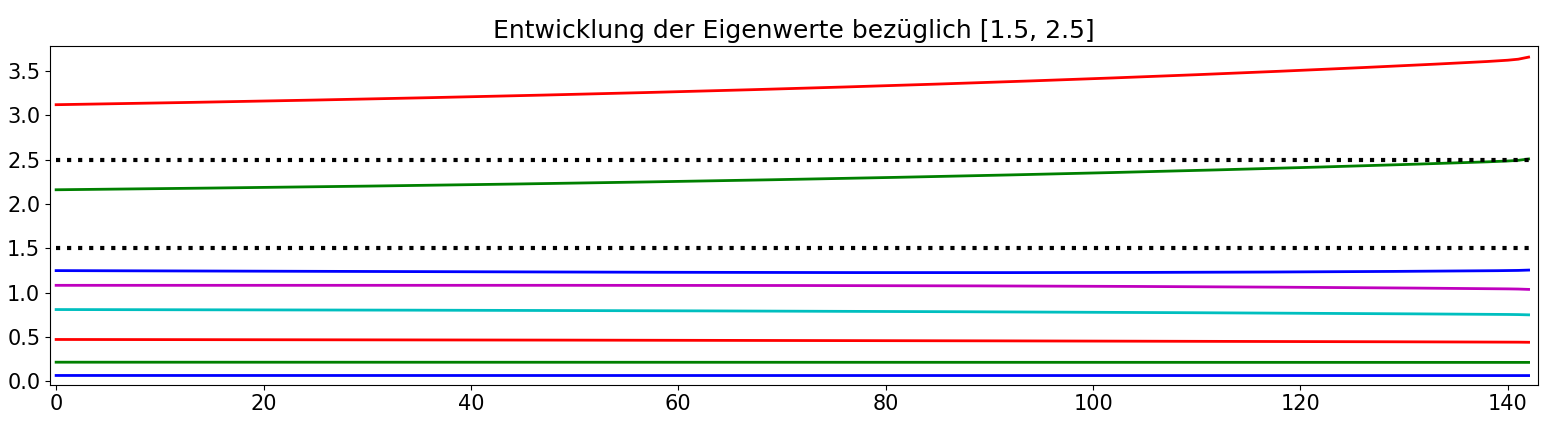
\includegraphics[width=0.9\textwidth, keepaspectratio]{./Mittelpunkt/Plot_1_100_0.05.png}
                  \caption{System 1, $m=100$, $\lambda_*=0.05$, Mittelpunkts-Regel verwendet}
                  \label{fig: Plot_1_100_0.05_Mittelpunkt}
            \end{figure}

            Der zweite Eigenwert verlässt in Abb. \ref{fig: Plot_1_100_0.05_Mittelpunkt} langsam das Intervall und hat keine Probleme die Intervallgrenze zu überqueren.
            Der Verlauf der Eigenwertzählungen ist hier zwar nicht abgebildet, aber an der Abwesenheit von Sprüngen kann man schließen, dass die approximiere gewichtete Eigenwertzählung die genaue hier überall gut approximiert. 
            Betrachte nun die Durchläufe zu System 1:

            \begin{figure}[h!t]
                  \centering
                  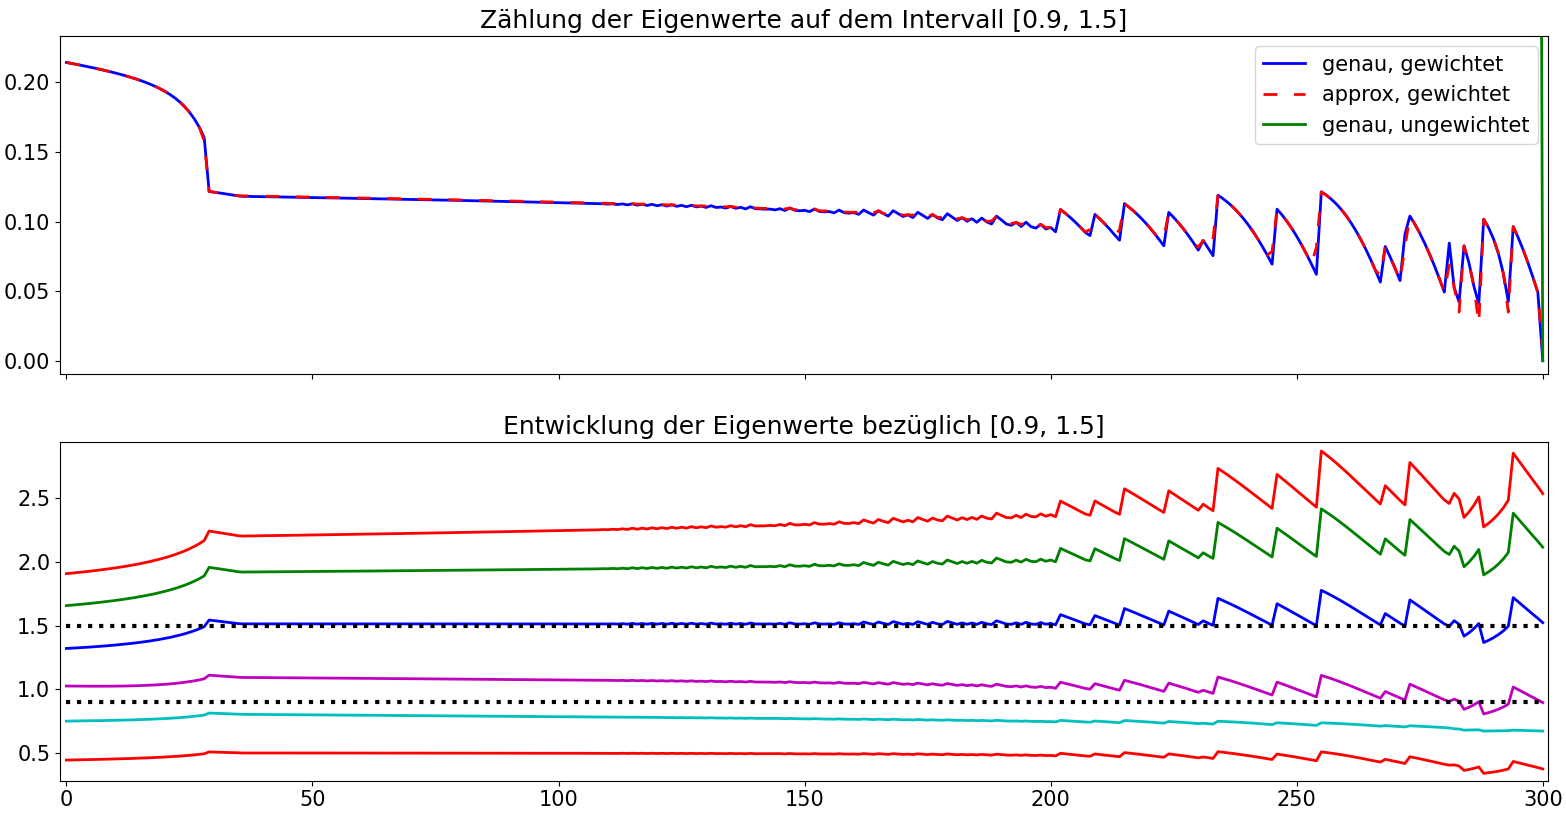
\includegraphics[width=0.9\textwidth, keepaspectratio]{./Mittelpunkt/Plot_2_100_0.05.png}
                  \caption[System 2, $m=100$, $\lambda_*=0.05$, Mittelpunkts-Regel]{System 2, $m=100$, $\lambda_*=0.05$, Mittelpunkts-Regel verwendet}
                  \label{fig: Plot_2_100_0.05_Mittelpunkt}
            \end{figure}

            In Abb. \ref{fig: Plot_2_100_0.05_Mittelpunkt} kann man sehen, dass immer Sprünge auftreten, wenn ein Eigenwert sich einer Intervallgrenze nähert und die Approximation der gewichteten Eigenwertzählung ungenau wird\footnote{siehe auch \cite[\textit{./Verbesserung\_Mittelpunkt.py}]{github}}.
            Weiterhin wird durch Ausführen des Programms klar, dass sich die Eigenwerte zwischen den Durchläufen von System 2 stark unterscheiden.
            Diese Instabilität der Minimierung kann nicht verhindert werden.
            Wir werden nun versuchen, die beobachteten Sprünge zu unterbinden. Nutze dazu eine genauere Quadraturformel.

            Nehme daher als zweites Beispiel die \zitat{Zweipunkt-Formel}\cite[S. 526]{numerikHermann}. Analog zu (\ref{def: JSternTrapez}) und (\ref{def: JSternMittel}) folgt:
            \begin{align}
                  J(s) \approx& \frac 1 {2\pi i}\left[\frac{\pi i \Tilde r}{m}\sum_{k=0}^{m-1}\klammer{L(z_{k,-}, s)\exp\klammer{-\frac{\pi i}{\sqrt{3}m}}+L(z_{k,+}, s)\exp\klammer{\frac{\pi i}{\sqrt{3}m}}}\right]\nonumber\\
                  =&: J^*_{\text{Gauss}}(s)
            \end{align}
            mit $z_{k,\pm}:=\Tilde z_0+\Tilde r\exp\klammer{\frac{\pi I}{\sqrt{3}m}(2\sqrt 3 k+\sqrt 3 \pm 1)}$

            Diese Formel erhält man durch Anwenden der Zweipunkt-Formel aus \cite[S. 526]{numerikHermann} und Einsetzen von
            $$u= \frac{a+b}{2} = \frac{2\pi}{m}(k+\frac 1 2)\text{ und }v=\frac{b-a}{2}=\frac \pi m$$

            Es folgen die Ergebnisse des Programms \textit{./Verbesserung\_Gauss2.py}.

            \begin{table}[!ht]
                  \centering
                  \begin{tabular}{lllcc}
                       System & $m$ & $\lambda_*$ & Iterationen & Zeit in s\\
                       \hline
                       1 & $100$ & $0.05$ & $145$ & $7.5$ \\ 
                       1 & $150$ & $0.05$ & $145$ & $10.3$ \\
                       \hline
                       1 & $100$ & $0.5$ & $15$ & $0.9$ \\
                       1 & $150$ & $0.5$ & $15$ & $1.1$ \\
                       \hline
                       2 & $100$ & $0.05$ & $112$ & $11.9$ \\
                       2 & $150$ & $0.05$ & $63$ & $9.3$ \\
                       \hline
                  \end{tabular}\\
                  \captionof{table}{Kennzahlen bei Verwendung der Zweipunkt-Formel}\label{tab: Ergebnisse_Gauss2}
            \end{table}

            Obwohl die Zweipunkt-Formel eine \zitat{Gaußsche Quadraturformel}\cite[S. 523]{numerikHermann} ist
            und damit einen optimalen Genauigkeitsgrad von 5 besitzt (vgl. \cite[S. 522f.]{numerikHermann}),
            so ist der Unterschied zur Mittelpunkts-Regel in den Durchläufen zu System 1 gering.
            Im Vergleich zu Tabelle \ref{tab: Ergebnisse_Mittelpunkt} bemerke man aber, dass sich die benötigten Zeiten bei System 1 verdoppelten.
            Dies war zu erwarten, wenn die doppelte Anzahl an Funktionswerten pro Teilintervall berechnet wird.
            In den Durchläufen zu System 2 kann aber festgestellt werden, dass sich die Anzahl an benötigten Iteration stark verringert.
            Betrachte dazu auch Abb. \ref{fig: Plot_2_100_0.05_Gauss2}.
            \begin{figure}[h!t]
                  \centering
                  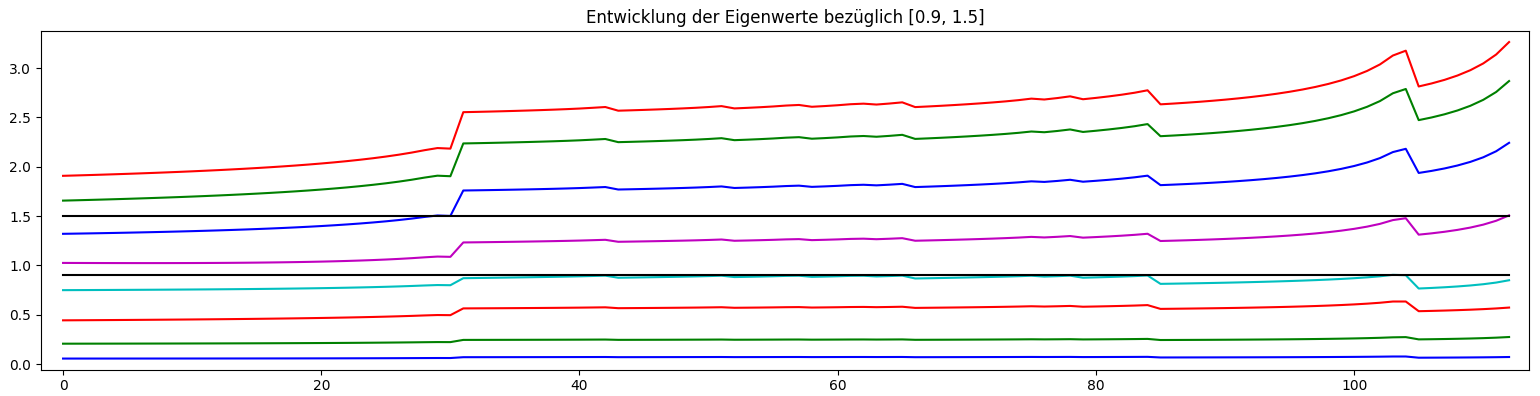
\includegraphics[width=0.9\textwidth, keepaspectratio]{./Gauss2/Plot_2_100_0.05.png}
                  \caption[Plot zu System 2, $m=100$, $\lambda_*=0.05$, Zweipunkt-Formel]{Plot zu System 2, $m=100$, $\lambda_*=0.05$, Zweipunkt-Formel verwendet}
                  \label{fig: Plot_2_100_0.05_Gauss2}
            \end{figure}

            Man sieht in Abb. \ref{fig: Plot_2_100_0.05_Gauss2}, dass sich die Eigenwerte hier von Anfang an schnell auf den Intervallrand zubewegen,
            im Gegensatz zu Abb. \ref{fig: Plot_2_100_0.05_Mittelpunkt}, wo die Eigenwerte sich in den Schritten 40 bis 200 wenig bis kaum veränderten.
            Durch die bessere Approximation kann trotz des erhöhten Rechenaufwands, der mit der Zweipunkt-Formel entsteht, die benötigte Zeit stark reduziert werden.
            Ferner kommt dazu, dass nun auch die Wahl von $m$ eine Rolle spielt: in den Tabellen \ref{tab: Ergebnisse_Mittelpunkt} 
            und \ref{tab: Ergebnisse_Gauss2} verringert sich die Anzahl an Iterationen bei erhöhter Anzahl an Stützstellen.
            Man nehme daher für die Minimierung der Eigenwerte in dem restlichen Kapitel immer die Zweipunkt-Formel.

            Die Tatsache, dass diese zwei Quadraturformeln nicht bei $\lam_a$ und $\lam_b$ ausgewertet werden und sie deshalb genauer sind,
            kann auch in Programm \textit{./Vergleich Quadraturformeln.py} gesehen werden.
            Dort wurde ebenfalls die verschobene Trapezregel betrachtet, welche die Stützstellen $z_{k+\frac 1 2}$ statt $z_k$ verwendet.
            Allein dies macht einen gewaltigen Unterschied:

            Für eine immer näher an das Kurvenintegral rückende Polstelle wächst die Approximation $J^*_{\text{Trapez}}$ aus (\ref{def: JSternTrapez}) sehr stark an.
            Alle anderen Quadraturformeln nähern sich stattdessen $0,5$.
            Wie auch in den Durchläufen zu System 1 liegen die Ergebnisse der Mittelpunkts-Regel und der Zweipunkt-Formel sehr dicht beieinander.

      \section{dynamische Schrittweite}
            Als nächstes wende man sich dem Gradientenverfahren zu:
            Die Schrittweite $\lambda_*$ soll nun nicht mehr fest sein, sondern möglichst optimal berechnet werden.

            Berechne daher $\nabla J^*(s_\text{neu})$ für $s_\text{neu} = s_\text{alt}-d*\lambda_*$\footnote{$d$ wie in Algorithmus \ref{alg: steilster Abstieg}} und entscheide aufgrund dessen, ob:
            \begin{itemize}
                  \item dieser Wert $(s_\text{neu})$ zurückgegeben wird,
                  \item der vorherige Wert $(s_\text{alt})$ zurückgegeben wird oder
                  \item man noch einen Schritt geht.
            \end{itemize}
            
            Offenbar bestimmt $\lambda_*$ nicht mehr direkt die Schrittweite, sie bestimmt aber die Entfernung zweier Punkte $s_\text{neu}$.

            Der Algorithmus zur Bestimmung des neuen Punktes ist in \cite[\textit{./Funktionen.py}]{github} in der Funktion \textit{schrittGradientenverfahren} definiert.

            Diese Funktion gibt einen Wert \s aus, der möglichst nahe an der optimalen Stelle bezüglich Richtung $d$ ist.
            Die optimale Stelle würde laut \cite[S. 286]{optimierungBurkhard}
            $$\nabla J(s)\cdot d^T = 0$$
            erfüllen, der nächste Schritt würde dann garantiert senkrecht auf diesem Schritt stehen.
            Da man nur eine endliche Zahl an Stellen auswerten kann, findet man diese Stelle fast sicher nicht.
            Daher soll die Bedingung
            $$|\nabla J(s)\cdot d^T| < 0.00001$$
            ausreichen.
            Es besteht weiterhin die Möglichkeit, dass $s$ die zulässige Menge $\Omega$ verlässt, oder man über einen optimalen Parameter springt.
            Auch diese Fälle werden in der Funktion \textit{schrittGradientenverfahren} behandelt.

            Das Anwenden dieses Algorithmus zur Bestimmung des nächsten Punktes bringt folgende Ergebnisse:
            \begin{table}[!ht]
                  \centering
                  \begin{tabular}{lllcc}
                       System & $m$ & $\lambda_*$ & Iterationen & Zeit in s\\
                       \hline
                       1 & $100$ & $0.05$ & $1$ & $10.4$ \\ 
                       1 & $150$ & $0.05$ & $1$ & $17.26$ \\
                       \hline
                       1 & $100$ & $0.5$ & $1$ & $1.8$ \\
                       1 & $150$ & $0.5$ & $1$ & $3.1$ \\
                       \hline
                       2 & $100$ & $0.05$ & $24$ & $16.7$ \\
                       2 & $150$ & $0.05$ & $178$ & $62.0$ \\
                       \hline
                  \end{tabular}\\
                  \captionof{table}{Kennzahlen bei Verwendung eines dynamischen Schrittweite}\label{tab: Ergebnisse_dynamischSchritt}
            \end{table}

            Die Ergebnisse sind auch in \cite[\textit{./Verbesserung\_dynamischeSchrittweite.py}]{github} zu finden.

            Wie man sehen kann, wird die Eigenwertzählung bei allen Durchläufen zu System 1 innerhalb eines Schrittes minimiert.
            Dies war aber zu erwarten, da $s$ in System 1 ein Skalar war.
            Sofern die Ableitung hier immer das gleiche Vorzeichen besitzt, gehen auch alle anderen Durchläufe aus Kapitel \ref{sec: Verbesserungen} bei System 1 immer nur in eine Richtung.
            Somit macht hier das Verfahren in einem Schritt, was vorher in $n$ Schritten gemacht wurde.

            Hier benötigt der zweite Durchlauf zu System 2 mehr Schritte als der der vergleichbare Durchlauf aus Tabelle \ref{tab: Ergebnisse_Gauss2} und die Minimierung dauert dabei noch länger,
            da jeder Schritt des Gradientenverfahrens hier zusätzlich aus Unterschritten (der Bestimmung des optimalen Parameters) besteht.

            Insgesamt lohnt sich eine dynamische Schrittweite in diesem Problem nicht, da keine einfache Möglichkeit besteht, die optimale Schrittweite zu bestimmen.
            Für die Bestimmung der optimalen Schrittweite werden hier die Schritte in die Richtung $d$ gegangen, aber schon nach dem ersten Schritt ist diese Richtung im Allgemeinen nicht optimal.
            Es kommt auch zu keiner Reduktion der Rechendauer, da nach jedem dieser Unterschritte wieder $\nabla J(s)$ bestimmt wird.

      \section{Approximation der Ableitung der gewichteten Eigenwertzählung}

            Zuletzt bemerke zuerst, dass die Approximation des Integrals durch die Quadraturformel die meiste Zeit benötigt,
            hingegen die genaue gewichtete Eigenwertzählung $J(s)$ sehr schnell berechnet werden kann.
            Da aber keine explizite Abhängigkeit vom Design-Parameter $s$ besteht, ist diese Formel nur gut, um als Bedingung für das Ende des Gradientenverfahrens zu dienen.

            Approximiert man aber $\nabla J$ durch die Anwendung eines Differenzenverfahren auf $J(s)$ aus (\ref{def: J original}),
            wie es in Kapitel \ref{sec: Programmieren} angewendet wurde, um $\frac {dM}{ds}$ zu approximieren,
            so kann diese Approximation genutzt werden, um die Berechnung von $\nabla J^*(s)$ und damit die Anwendung der Quadraturformel zu umgehen
            \footnote{man ersetzt also die Ableitung der Approximation von $J$ durch die Approximation der Ableitung von $J$}.

            Da diese Berechnung sehr viel schneller ist, erhöhe die maximal mögliche Anzahl an Iterationen pro Durchlauf auf 100000.
            Die Anzahl an Teilintervallen wird zwar nicht für die Berechnung an sich benötigt, aber bei jeder Iteration des Gradientenverfahrens wird für den aktuellen Wert des Design-Parameters $s$
            ein entsprechendes $J^*(s)$ berechnet und gespeichert, um den Verlauf der approximierten gewichteten Eigenwertzählung in dem oberen Plot abzubilden.
            Um diesen Mehraufwand so gering wie möglich zu halten sei $m=1$. Die approximierte gewichtete Eigenwertzählung wird dadurch zwar sehr ungenau,
            aber hier wird sie für keinen Schritt des Gradientenverfahrens verwendet.
            Nehme daher für System 1 nicht vier Durchläufe, sondern nur zwei, da die Unterscheidung bezüglich $m$ entfällt.
            Den vierten Durchlauf findet man zwar nicht in dem Programm \mbox{\cite[\textit{./Verbesserung\_NablaJ.py}]{github}}, man kann ihn aber durch Veränderung des Werts von Argument \zitat{maxIter} in Zeile 15 berechnen lassen.
            Dieser Durchlauf wird nicht immer durchgeführt, da er zu viel Zeit in Anspruch nehmen.
            Die folgenden Ergebnisse können auch in \mbox{\textit{./Verbesserung\_NablaJ.py}} wiedergefunden werden.

            \begin{table}[!ht]
                  \centering
                  \begin{tabular}{lllcc}
                       System & $m$ & $\lambda_*$ & Iterationen & Zeit in s\\
                       \hline
                       1 & $1$ & $0.05$ & $31$ & $0.03$ \\ 
                       \hline
                       1 & $1$ & $0.5$ & $4$ & $0.01$ \\
                       \hline
                       2 & $1$ & $0.05$ & $>100000$ & $>198$ \\
                       2 & $1$ & $0.05$ & $>150000$ & $>630$ \\
                       \hline
                  \end{tabular}\\
                  \captionof{table}{Kennzahlen bei Verwendung von $\nabla J(s)$}\label{tab: Ergebnisse_nablaJ}
            \end{table}

            Man beachte, dass diese Approximation für System 1 genau genug war, um ein Minimum innerhalb von 0.03 s zu finden.
            Allerdings ist dieses Verfahren in dieser Form für System 2 unzureichend. Man könnte die Ableitung genauer approximieren,
            indem die Schrittweite $h$ aus (\ref{def: DiffVerfahren}) verringert.
            Ferner würde vielleicht eine größere Schrittweite $\lambda_*$ helfen, um (ähnlich wie bei System 1) die Anzahl an Iterationen zu verringern.
            Solche Überlegungen werden in dieser Arbeit aber nicht weiter ausgeführt.

            Für die Durchläufe für System 2 erkenne man auch, dass die Zeit nun nicht mehr proportional zu den gegangenen Schritten ist.
            Dies liegt wahrscheinlich daran, dass nicht mehr alle Werte im Arbeitsspeicher gespeichert werden konnten, wodurch sich die Zugriffszeiten verlängern.

            Diese Variante hat somit zwar sehr viel Potenzial (siehe Durchläufe zu System 1), ist aber in der jetzigen Form nicht für alle Probleme genau genug.

\chapter{Auswertung}
\label{sec: Auswertung}

      In dieser Arbeit wurden in Kapitel \ref{sec: EW Problem_Futamura} der Matrix-Pencil, die Eigenwerte eines Matrix-Pencils,
      die allgemeine Schur-Zerlegung und die Identität von Futamura vorgestellt.
      Während die Schur-Zerlegung für den Beweis der Identität von Futamura benötigt wird, liefert sie auch eine Aussage über die Eigenwerte des Matrix-Pencils.
      Diese Identität erlaubt eine direkte Aussage über die Anzahl an Eigenwerten in einem Intervall, dafür muss aber ein Kurvenintegral berechnet werden.

      In Kapitel \ref{sec: MS Matrizen} wurden die Systeme vorgestellt, welche in Kapitel \ref{sec: Programmieren} und \ref{sec: Verbesserungen} behandelt werden.
      Um die Eigenwerte dieser Systeme zu berechnen, wurden die Massen- und Steifigkeitsmatrizen der Systeme berechnet und eine Formel für die Berechnung der Eigenkreisfrequenzen aufgestellt.
      Durch eine Substitution in dieser Formel erhält man in (\ref{eqn: allg EW Problem mit lam}) die Formel für die Eigenwerte des Matrix-Pencils $(K-\lambda M)$.

      In Kapitel \ref{sec: EW Zählung} wurde die gewichtete Eigenwertzählung auf einem Intervall hergeleitet. Diese Funktion besitzt die Form aus (\ref{def: J original})
      und ist einfach zu berechnen, hängt aber nicht direkt von dem Design-Parameter Verwendung findet.

      Durch die Identität von Futamura, dem Residuensatz und einer Quadraturformel erhält man in (\ref{def: JSternTrapez}) eine Approximation dieser Eigenwertzählung,
      welche direkt von $s$ abhängt.

      Diese Approximation wird in Kapitel \ref{sec: Programmieren} genutzt, um die Eigenwerte der Systeme auf einem Intervall zu zählen und anschließend zu eliminieren.
      
      Als Quadraturformel wurde in Kapitel \ref{sec: Programmieren} die normale Trapezregel verwendet, welche aber unzureichende Ergebnisse brachte (siehe Tabelle \ref{tab: Ergebnisse}).

      Unter anderem wurde in Kapitel \ref{sec: Verbesserungen} diese Problem behoben.
      Auch wurde in Kapitel \ref{sec: Verbesserungen} das Gradientenverfahren aus Algorithmus \ref{alg: steilster Abstieg} weiterentwickelt, sodass die Schrittweite nun dynamisch berechnet wird.
      Durch mangelnde Möglichkeiten, diese Schrittweite effizient zu berechnen, war dieses Verfahren nicht so effektiv wie das in Kapitel \ref{sec: Programmieren} vorgestellte Gradientenverfahren.

      Zuletzt wurde in Kapitel \ref{sec: Verbesserungen} auch eine Approximation der Ableitung von $J(s)$ eingeführt.
      Diese kann zwar die Eigenwertzählung von System 1 unglaublich schnell minimieren, sie versagte aber bei einem mehrdimensionalen Design-Parameter, wie er in System 2 genutzt wird.

      Der schnellste Weg zur Minimierung der Eigenwertzählung ist daher eine möglichst genaue Quadraturformel,
      welche möglichst wenig Stützstellen benötigt, um ein gutes Ergebnis mit geringstem Zeitaufwand zu erhalten.

      Für eindimensionale Design-Parameter kann das Verfahren durch die Approximation von $\nabla J(s)$ stark beschleunigt werden.
      Für einen Parameter $\s\in \R^l, l>1$ kann diese Approximation auch weiterhelfen, allerdings wurde dieser Ansatz für mehrdimensionale Parameter nicht weiter verfolgt.

      Für alle Design-Parameter kann aber die Funktion $\nabla J^*$ mit einer entsprechend genauen Quadraturformel verwendet werden, um die Eigenwertzählung kontrolliert zu minimieren.
      Dieses Verfahren dauert zwar länger, bringt aber verlässlich gute Ergebnisse (siehe Tabelle \ref{tab: Ergebnisse_Mittelpunkt} und \ref{tab: Ergebnisse_Gauss2}).

      Es gibt aber offenbar noch andere Möglichkeiten die Minimierung zu beschleunigen.
      Man könnte einerseits ein anderes Minimierungsverfahren nutzen, wie das Newton-Verfahren (siehe \cite[S. 290]{optimierungBurkhard}).
      Für dieses Verfahren bräuchte man zwar die zweite Ableitung von $J$ oder $J^*$, es könnte sich aber positiv auf die Rechenzeit auswirken.

      Zudem könnte man für Systeme mit einer hohen Anzahl an Freiheitsgraden die Spur aus $L(z,s)$, wie es in (\ref{eqn: vollständigeAblL}) vorkommt, approximieren.
      Man erhofft sich dadurch, die Komplexität der Funktion und ebenso die benötigte Zeit zu verringern (vgl. \cite[S. 128]{grundlageFutamura}).
      Dazu wäre Hutchinson's Schätzer (vgl. \cite[S. 142]{hutch++Meyer}), oder dessen Erweiterung \zitat{Hutch++}\cite[S. 142]{hutch++Meyer} nützlich.
      Solche Überlegungen könnten in einer weiterführenden Arbeit behandelt und mit den hier erhaltenen Ergebnissen verglichen werden.

\chapter{Verzeichnisse}
      \printbibliography
      \printacronyms[name=Abkürzungsverzeichnis, include={abbrev}]
      %%
      %% Erscheint auf letzter Seite
      %%
      \chapter*{Erkl\"{a}rung}
      \thispagestyle{empty}
      Hiermit erkl\"{a}re ich, dass ich die am \datum\ eingereichte Bachelorarbeit zum Thema
      \emph{\thema} unter Betreuung von \betreuer\ selbstst\"{a}ndig erarbeitet,
      verfasst und Zitate kenntlich gemacht habe. Andere als die angegebenen Hilfsmittel
      wurden von mir nicht benutzt.

      \bigskip \bigskip \bigskip \bigskip \bigskip

      Dresden, \datum\ \hfill Unterschrift

      \normalsize
\end{document}